\documentclass[oneside, 12pt]{book}
%\renewcommand*\familydefault{\sfdefault} 
\usepackage[activeacute, spanish]{babel}
\usepackage[utf8]{inputenc}
\usepackage{titlesec}
\usepackage[left=2cm, right=2cm, bottom=3cm]{geometry}
\usepackage{graphicx}
\usepackage{amssymb}
\usepackage{float}
\usepackage{slashbox}
\usepackage[hidelinks]{hyperref}
\usepackage{fancyhdr}
%\usepackage[scaled]{helvet}
%\renewcommand\familydefault{\sfdefault} 
%\usepackage[T1]{fontenc}
\linespread{1}%para texto a espacio y medio \textheight=24cm

\begin{document}
	
	\frontmatter
	
	\begin{titlepage}
	 	\begin{center}	 		
	 		%``''
		   	
		   	\vskip 0.75cm
		  	{\normalsize{\bf UNIVERSIDAD ANDINA NÉSTOR CÁCERES VELÁSQUEZ}}

		  	{\normalsize{\bf FACULTAD DE INGENIERÍA DE SISTEMAS}}

			{\normalsize{\bf C.A.P INGENIERÍA DE SISTEMAS}} 
			\vskip 0.75cm
			\begin{figure}[htb]
			    \centering
				
\includegraphics[width=6cm, height=7cm]{../imgs/ESCUDO_UANCV.jpg}
			\end{figure}
		    \vskip 0.75cm
		    
		   	{\large{\bf INFORME DE PRÁCTICAS PRE-PROFESIONALES}}\\
		   	\vskip 1cm
		   	
		    Prácticas realizadas en:\\
		    
		    {\bf WELL DONE SOLUTIONS SAC}\\		  
		    \vskip 1cm
		    
		   	Elaborado por:\\
		   	
		   	{\bf MAMANI PAUCAR, wilder}\\
		   	
		   	\vskip 1cm
		   	
		   	{\normalsize{\bf PARA OPTAR EL GRADO DE BACHILLER EN INGENIERÍA DE
		   	SISTEMAS}}\\
		   	
		   	\vskip 2cm
		    
		   	{JULIACA - PERU}\\{2018}
	 	\end{center}
	\end{titlepage}		
	
	% Configuracion del documento
		\newcommand{\bigrule}{\titlerule[0.5mm]}
		\titleformat{\chapter}[display] % cambiamos el formato de los capitulos
		{\bfseries\Huge} % por defecto se usaran caracteres de tamaño \Huge en negrita
		{% contenido de la etiqueta
			 \titlerule % linea horizontal
			 \filleft % texto alineado a la derecha
			 %\Large\chaptertitlename\ % ``Capitulo'' o ``Apendice'' en tamaño \Large en
			 % lugar de \Huge \Large\thechapter % numero de capitulo en tamaño \Large
		 }
		{0mm} % espacio minimo entre etiqueta y cuerpo
		{\filleft} % texto del cuerpo alineado a la derecha
		[\vspace{0.5mm} \bigrule] % despues del cuerpo, dejar espacio vertical y
		% trazar linea horizontal gruesa
		
		
	% Configuracion para encabezados y pie de pagina
		\renewcommand{\chaptermark}[1]{\markboth{\MakeUppercase{\thechapter. #1 }}{}}
		\renewcommand{\sectionmark}[1]{\markright{\thesection\ #1}}
		\fancyhf{}
		%\fancyhead[RO]{\bfseries\rightmark}
		%\fancyhead[LE]{\bfseries\leftmark}
		\fancyhead[RO]{\rightmark}
		\fancyhead[LE]{\leftmark}
		\fancyfoot[C]{\thepage}
		\renewcommand{\headrulewidth}{0.5pt}
	
		\addtolength{\headheight}{0.5pt}
		\fancypagestyle{plain}{
		  \fancyhead{}
		  \renewcommand{\headrulewidth}{0pt}
		}
	
	% Dedicatoria	
	\newpage
	\pagestyle{empty}
	\vspace*{17cm}
	\begin{flushright}\itshape
		A mi Familia por enseñarme el camino correcto.
	\end{flushright}
	
	\newpage
	
	\renewcommand\contentsname{Índice General}
	\renewcommand\listfigurename{Índice de figuras}
	
	\listoffigures
	\listoftables
	\tableofcontents % Tabla de contenido
	\mainmatter
	\pagestyle{fancy}
	% Presentacion
	\chapter{Presentación}
	\section{Objetivo del Informe}
		Aplicar los conocimientos adquiridos durante los cinco años de formación
		profesional dentro de la carrera académico profesional de {\bf Ingeniería de
		Sistemas} de la  {\bf ``Universidad Andina Néstor Cáceres Velásquez''} de la
		ciudad de Juliaca.
	
	\section{Periodo de Prácticas Pre Profesionales}
		Periodo de prácticas realizadas: {\bf 1 de septiembre del 2015} - {\bf 29 de
		febrero del 2016}.
		
	\section{Institución y Área de Trabajo} 
		Las prácticas se realizaron en la empresa {\bf ``Well Done Solutions SAC''} en
		el área de {\bf Desarrollo de Software}.
		
	\section{Funciones del Área de Trabajo}
		El Área de trabajo se dedica netamente al desarrollo de software a medida.
		
		\subsection{Planificar, organizar, diseñar e implementar software a medida}
			La mayoría de las empresas aún usan sistemas de información manuales, siendo
			una limitante de cara a aquellas empresas que hacen uso intesivo de sistemas
			automatizados; a esto se suma la necesidad de agilizar procesos de negocios y
			entregar información precisa a usuarios y clientes. Brindamos soluciones de
			software a medida, haciendo uso de tecnologías emergentes en el mundo del desarrollo de software.

			

	\chapter{Datos Generales del Practicante}
	
	\begin{tabular}{ p{8cm} p{8cm} }
		{\bf APELLIDOS Y NOMBRES} & : Mamani Paucar, wilder \\\\
		{\bf DOMICILIO ACTUAL} & : Jr. Mariano Melgar \#657 \\\\
		{\bf DNI} & : 73529058 \\\\
		{\bf CELULAR} & : 951-503-009 \\\\
		{\bf ÁREA DE TRABAJO} & : Desarrollo de Software \\\\
		{\bf CARGO} & : Analista Programador \\\\
		{\bf EMAIL} & : \href{mailto:w11ld33r@gmail.com}{w11ld33r@gmail.com} \\\\
		{\bf GITHUB} & :
		\href{https://www.github.com/w11ld33r}{https://www.github.com/w11ld33r}
	\end{tabular}
	\chapter{Aspectos Generales de la Empresa}

	\section{Descripción}
		\begin{itemize}
			\item {{\bf WELL DONE SOLUTIONS SAC} es una empresa privada ubicada en la
			ciudad de Juliaca, Departamento de Puno, Perú}
			\item {Inició su funcionamiento el 5 de Octubre  del año 2014}
		\end{itemize}
		
	\section{Ubicación}
		Pasaje $1^{ero}$ de Mayo 112 - Oficina 301
		
	\section{Teléfono}
		051 33-6975
		
	\section{Portal Web}
		\href{http://www.wdsolutions.pe}{http://www.wdsolutions.pe}
	
	\section{Actividades que Realiza}
		La empresa {\bf ``Well Done Solutions SAC''} se dedica a brindar asesoría,
		desarrollo de software, cursos talleres, mantenimiento de servidores, entre
		otros servicios relacionados a la tecnología.
	
		\subsection{Desarrollo de software}
			Como se mencionó anteriormente, la empresa brinda soluciones de
			software a medida, haciendo uso de tecnologías emergentes en el mundo del desarrollo de software.
			
		\subsection{Cursos presenciales}
			La mayoría de jovenes tanto recien egresados como autodidactas, muchos de
			ellos solo aprendieron a construir programas sencillos y no saben como
			enfrentarse a proyectos reales. La empresa  {\bf ``Well
			Done Solutions SAC''} dicta cursos presenciales al público en general,
			quienes quieran aprender o reforzar conocimientos de las últimas tendencias
			en lenguajes de programación o arquitectura de software, entre otros.
			
		\subsection{Creación de portales corporativos}
			Tener presencia en internet es la mejor forma de darse a conocer ante mundo.
			Empresas privadas como públicas buscan tener dicha presencia para dar a
			conocer los productos o servicios que brindan.
			{\bf ``Well Done Solutions SAC''} brinda servicios de creación de portales
			corporativos a medida.

	\chapter{Actividades Realizadas}
	En el área de desarrollo de software colaboré en las distintas etapas del
	desarrollo del sistema que se desarrolló. Reuniones con usuarios para la
	obtención de requisitos, análisis de requisitos, diseño del sistema, desarrollo
	del sistema y por último puesta en producción del sistema.\\\
	
	A lo largo del periodo de prácticas utilice herrmientas que ayudan a ser
	productivos, tales son: Sistemas de control de versiones (Git, Bitbucket,
	Github, Gitlab), Entornos de Desarrollo Integrado (Eclipse, Netbeans, IntelliJ
	IDEA, Spring Tool Suite), editores de texto (Sublime Text, Atom, Visual Studio Code, Brackets), etc.
	
	\section{Obtención de requisitos}
		La obtención de requisitos es la etapa inicial y fundamental de cualquier tipo
		de proyecto de software que se quiera realizar. Se enfocan sólo en la visión
		del sistema que tiene el usuario. La funcionalidad del sistema, la interacción entre el
		usuario y el sistema, los errores que el sistema puede detectar y manejar son
		parte de los requisitos \cite{bernd1ingenieria}.
		
		La obtención de requerimientos incluye las siguientes actividades:
		
		\begin{itemize}
		  \item {\bf Identificación de actores.} {Durante esta actividad se
		  identifican los diferentes tipos de usuario que el sistema soportará.}
		  
		  \item {\bf Identificación de escenarios.} {Aquí se observan a los futuros
		  usuarios y se desarrollan un conjunto de escenarios posibles para las
		  distintas funcionalidades del sistema.}
		  
		  \item {\bf Identificación de casos de uso.} {Una vez de acuerdo el usuario
		  con el equipo de desarrollo, se abstraen los escenarios en casos de uso.}
		\end{itemize}
		
		Hubo reuniones con los usuarios, escuchándolos activamente, proponiendo ideas,
		debatiendo, descartando casos de uso innecesarios. Para llegar a un acuerdo.
		Dentro de esta labor el equipo tenía un panorama general de todo el sistema y a su vez
		en cada reunión se tenía ideas y modelos de funcionalidades listas para
		implementar; y presentarlos en la próxima reunión para ser aprobado por los
		interesados del proyecto.\\\
		
		Esta labor se me fue encomendada a medida que me iba familiarizando con el
		equipo, ya que es una parte crítica de un proyecto de software.
	
	\section{Análisis de requisitos}
		El análisis de requisitos se enfoca en la producción de un modelo del sistema.
		El análisis de requisitos le proporciona al diseñador del sistema una
		representación de información y función \cite{pressman06ingenieria}. Aunque puede ser que el
		modelo de análisis no sea comprensible para los usuarios, ayuda a que los
		diseñadores del sistema verifiquen la especificación del sistema producida
		durante la obtención de requisitos.
		
		El análisis de requisitos produce tres modelos individuales:
		
		\begin{itemize}
		  \item {\bf Modelo funcional.} {Representado por casos de uso y escenarios.}
		  
		  \item {\bf Modelo de objetos de análisis.} {Representado por diagramas de
		  clase y objetos.}
		  
		  \item {\bf Modelo dinámico.} {Representado por diagramas de estado y de
		  secuencia.}
		\end{itemize}
		
		Fui partícipe de esta actividad progresivamente, opinaba de acuerdo a los
		conocimientos que tenía, pero el equipo siempre estuvo dispuesto a ayudarme,
		con lo cual despejaba dudas e inquietudes.
		
	\section{Diseño de software}
		El Diseño de software es un proceso mediante el cual los requisitos se
		convierten en un plano para construir el software. Al inicio el plano
		representa una visión general del software. A medida que se va avanzando el
		proceso, se van representado partes del software a profundidad.\\\
		
		Parte del diseño de software se encarga de describir la descomposición en
		subsistemas desde el punto de vista de responsabilidades, dependencias, flujo
		de control, control de acceso y almacenamiento de datos.\\\
		
		Forme parte de esta labor activamente, ya que tenía un buen conocimiento
		acerca de patrones de diseño, bases de datos, descomposicion de sistemas, etc.
		
		
	
	\section{Desarrollo Frontend y Backend}
		La parte de programación, es donde utilizamos todos los diseños y diagramas
		para empezar a codificar en algún lenguaje de programación. El desarrollo
		frontend y backend requiere de habilidades y conceptos como: conocimientos
		de algoritmos, estructuras de datos, pruebas unitarias, pruebas end-to-end, integración
		continua, etc.\\\
		
		Ingresé a la empresa desarrollando únicamente en el lado del frontend,
		conforme avanzaba en conocimientos, comencé a desarrollar frontend y backend,
		los cuales me permitieron conocer las tecnologías actuales que dominan el mercado
		del desarrollo de software empresarial.
		
		
	
	\section{Despliegue de sistemas en la Nube (vps)}	
		En esta última actividad se pone en producción el sistema en su totalidad.
		Servicios como \textit{Google Cloud Platform, Digital Ocean, Amazon Web
		Services, etc}, requieren de habilidades de administración de servidores que
		ofrecen estas empresas. Distino a un hosting compartido, las plataformas como
		\textit{Google Cloud Platform} brindan un espacio de almacenamiento dedicado
		exclusivo y la libertad de configurar el servidor de acuerdo a necesidades
		específicas. También permite escalar a medida que el sistema crece.\\\
		
		Gracias a los conocimientos en servidores linux pude asumir esta tarea, la de
		configurar, instalar paquetes y dejar todo listo para el funcionamiento
		correcto en la nube.\\\
		
		\textit{Conforme el proyecto avanzaba, pude desenvolverme adecuadamente en
		todas las actividades mencionadas.}

	\chapter{Descripción del Proyecto Realizado}
	Durante el periodo de prácticas se desarrolló un Sistema de Salud Ocupacional
	(basado en web), realizando un trabajo en equipo; por lo que el practicante
	estaba a cargo del desarrollo de ciertas funcionalidades del proyecto.
	
	\section{Objetivo}
		Análisis, Diseño e Implementación de un Sistema de Salud Ocupacional para la
		Clínica Del Valle de la ciudad de Juliaca.
		
	\section{Justificación}
		El sistema es necesario para la Clínica del Valle, porque les permitirá
		ahorrar tiempo y recursos, como también reducirá la tasa de errores; es necesario para
		los pacientes, porque se les brindará un servicio más rápido y con resultados
		precisos.
		
	\section{Planificación}
		La construcción del sistema tuvo una duración aproximada de seis meses. La
		planificación era flexible en cuanto a reuniones (cada dos semanas) con el
		cliente. Se llevó a cabo una primera reunión con el cliente, quién
		requería las funcionalidades primordiales/urgentes del sistema. Pasada las dos
		semanas se tenia un producto mínimo viable y funcional. Las iteraciones nos
		permitía ír añadiendo más funcionalidades.
		
	\section{Metodología}
		Se usó una metodología ágil apoyado en el conjunto de ideas que nos brinda
		``kanban'' y el Análisis y Diseño Orientado a Objetos.
		\section{Equipo de Desarrollo}
	\subsection{Gerente de Proyecto}
		\begin{itemize}
			\item El Gerente de proyecto coordina con el usuario líder
			\item Monitorea el desempeño de los recursos y tomara acciones correctivas
			\item Mantiene informado al usuario líder, actúa como enlace entre el
			personal del proyecto y otros tomadores de decisiones
		\end{itemize}
		
	\subsection{Jefe de Proyecto}
		
		El jefe de proyecto asigna los recursos, gestiona las prioridades, coordina las
		interacciones con los clientes y usuarios, y mantiene al equipo del proyecto
		enfocado en los objetivos. El jefe de proyecto también establece un conjunto de
		prácticas que aseguran la integridad y calidad de los artefactos del proyecto.
		Además, el jefe de proyecto se encargará de supervisar el establecimiento de la
		arquitectura del sistema. Gestión de riesgos. Planificación y control del
		proyecto.\\\
		
		El Jefe de Proyecto tiene las siguientes características:
		
		\begin{itemize}
			\item Experiencia en el diseño y desarrollo de aplicaciones Internet
			(Intranet/Extranet)
			
			\item Experiencia Liderando proyectos Internet
			
			\item Dominio de las metodologías más eficaces para el análisis de la
			información
			
			\item Ha participado en distintos proyectos dirigiendo y cumpliendo otro
			tipo de perfiles lo que hacen de él un elemento con la capacidad de
			distribuir las tareas de un proyecto
			
			\item Posee también, conocimientos especializados en áreas específicas del
			proyecto como puede ser: diseño, implantación y administración de Bases de
			Datos, servidores Web
		\end{itemize}
	
	\subsection{Analista de Sistemas}
		El Analista de Sistemas es la persona encargada de la captura, especificación y
		validación de requisitos, interactuando con el cliente y los usuarios mediante
		entrevistas. Elabora el Modelo de Análisis y Diseño. Colabora en la elaboración
		de las pruebas funcionales y el modelo de datos.
		
	\subsection{Arquitecto de Software}
		El Arquitecto es el encargado de definir el esquema de trabajo, la
		tecnología, gestión de requisitos, gestión de configuración e impactoen los
		cambios.
		
	\subsection{Analista Programador}
		El Analista Programador está encargado de la construcción de prototipos,
		desarrollo de los componentes. Colabora en la elaboración de las pruebas
		funcionales y en las validaciones con el usuario.\\\
		
		Dentro de este perfil tenemos los siguientes:
		
		\subsubsection{Analista Programador Junior}
			\begin{itemize}
				\item Egresado de la Universidad
				\item Conocimientos en Tecnología JAVA
				\item Conocimientos en Desarrollo JAVA
				\item Capacidad para trabajar en equipo
			\end{itemize}
			
		\subsubsection{Analista Programador Estándar}
			\begin{itemize}
				\item Egresado de la Universidad
				\item Experiencia en Análisis, Diseño y Desarrollo
				\item Conocimientos en Tecnología JAVA
				\item Experiencia en desarrollo JAVA (2 años)
				\item Capacidad para trabajar en equipo
			\end{itemize}
			
		\subsubsection{Analista Programador Senior}
			\begin{itemize}
				\item Egresado de la Universidad
				\item Experiencia en Análisis, Diseño y Desarrollo
				\item Conocimientos en Tecnología JAVA
				\item Conocimientos de arquitecturas
				\item Conocimiento de frameworks
				\item Experiencia en desarrollo JAVA (+4 años)
				\item Capacidad para trabajar en equipo
			\end{itemize}		
	
	\subsection{Programador}
		El programador es aquel que posee una amplia experiencia en desarrollo de
		aplicaciones Internet. Posee un criterio amplio y experiencia necesaria para
		el desarrollo de las aplicaciones del proyecto, de manera que resulten ser
		óptimas en tiempo de ejecución y uso de recursos.\\\
		
		Se encarga de investigar aquellos puntos del proyecto que necesiten una mejor
		visión, de manera que encuentre la mejor alternativa de solución que colabore
		con un óptimo desarrollo del proyecto. Tiene una base sólida en el
		conocimiento de sistemas operativos, herramientas de conectividad y
		desarrollo sobre distintas bases de datos, lo que le permite cumplir con los
		requerimientos del proyecto de manera eficaz.\\\
		
		Posee el conocimiento de las últimas herramientas de desarrollo en Internet,
		de manera que pueda utilizarlas eficientemente durante el desarrollo de sus
		aplicaciones.
		
	\subsection{Administrador de Bases de Datos}
		El Administrador de Base de Datos se encarga de autorizar el acceso a
		la base de datos, de coordinar y vigilar su empleo, se encarga de la
		instalación y configuración de los motores de Base de datos. Realiza además
		las siguientes funciones:
		
		\begin{itemize}
			\item Mejoras a los motores de Base de Datos.
							
			\item Manejo de seguridad: a nivel de Base de Datos definiendo la estructura y
			sus objetos (tablas, campos, procedimientos, usuarios, roles, triggers, etc.), y
			a nivel de usuarios definiendo el acceso de los diferentes usuarios a los
			objetos de la Base de Datos
			
			\item Monitoreo del espacio físico y los archivos lógicos para optimizar la Base
			de Datos
			
			\item Respaldos y Recuperación de Información
			\item Transferir e Importar Datos y estructuras de Base de Datos externas
			\item Mantenimiento a la Base de Datos
			\item Implementación de Réplicas
		\end{itemize}
		
	\subsection{Diseñador}
		Diseña la interfaz de la aplicación, trabaja desde el análisis para tener una
		visión integral del proyecto. Analiza la situación, define la estrategia de 	
		comunicación, la estructura lógica del site, la arquitectura de la
		información, jerarquiza los contenidos de acuerdo a su importancia. Define el
		estilo gráfico y de sus principales páginas aprovechando al máximo todas las
		herramientas de comunicación en Internet.
		
	\subsection{Documentador}
		Elabora todos los documentos requeridos para el sistema.
		\section{Análisis del Sistema}
	Se requiere un Sistema de Salud Ocupacional donde se puedan registrar
	empresas, pacientes (asociados o no a una empresa) que, deben ser sometidos a
	pruebas médicas de acuerdo a un perfil de exámenes previamente registrados.
	Terminada las pruebas, el sistema debe imprimir dichas pruebas junto con los
	datos calculados automáticamente.\footnote{El párrafo es un resumen del
	documento de requerimientos real.} \\\

	A continuación se muestran algunos diagramas:
	
	\begin{figure}[ht!]
	    \centering
		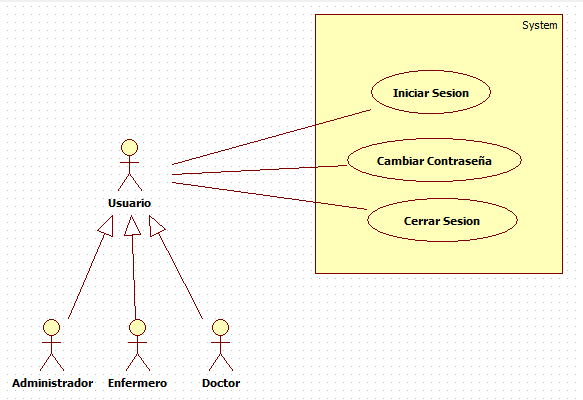
\includegraphics{../imgs/casos-uso/1.png}
		\caption{CU-1 Seguridad}
	\end{figure}
	
\newpage
	
	\begin{figure}[ht!]
	    \centering
		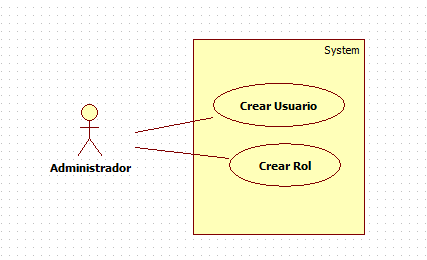
\includegraphics{../imgs/casos-uso/2.png}
		\caption{CU-2 Creación de Usuarios}
	\end{figure}
	
	\begin{figure}[ht!]
	    \centering
		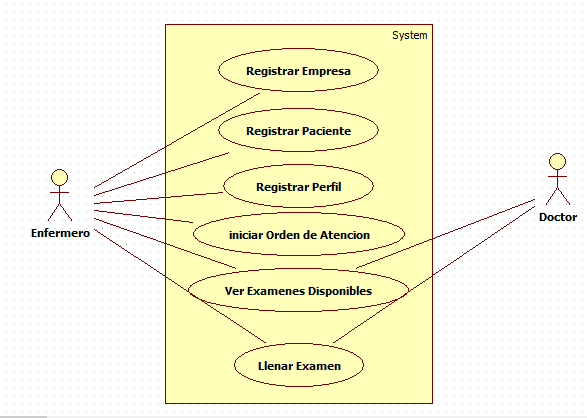
\includegraphics{../imgs/casos-uso/3.png}
		\caption{CU-3 Casos de Uso primordiales}
	\end{figure}
		\newpage
\section{Diseño del Sistema}
	A continuación se muestra parte del diagrama de clases y el diagrama de
	procesos (BPM):\footnote{Se puede encontrar los diagramas completos y legibles
	en
	\href{https://www.github.com/w11ld33r/informe-practicas/tree/master/imgs}{https://www.github.com/w11ld33r/informe-practicas/tree/master/imgs}}

	\begin{figure}[H]
	    \centering
		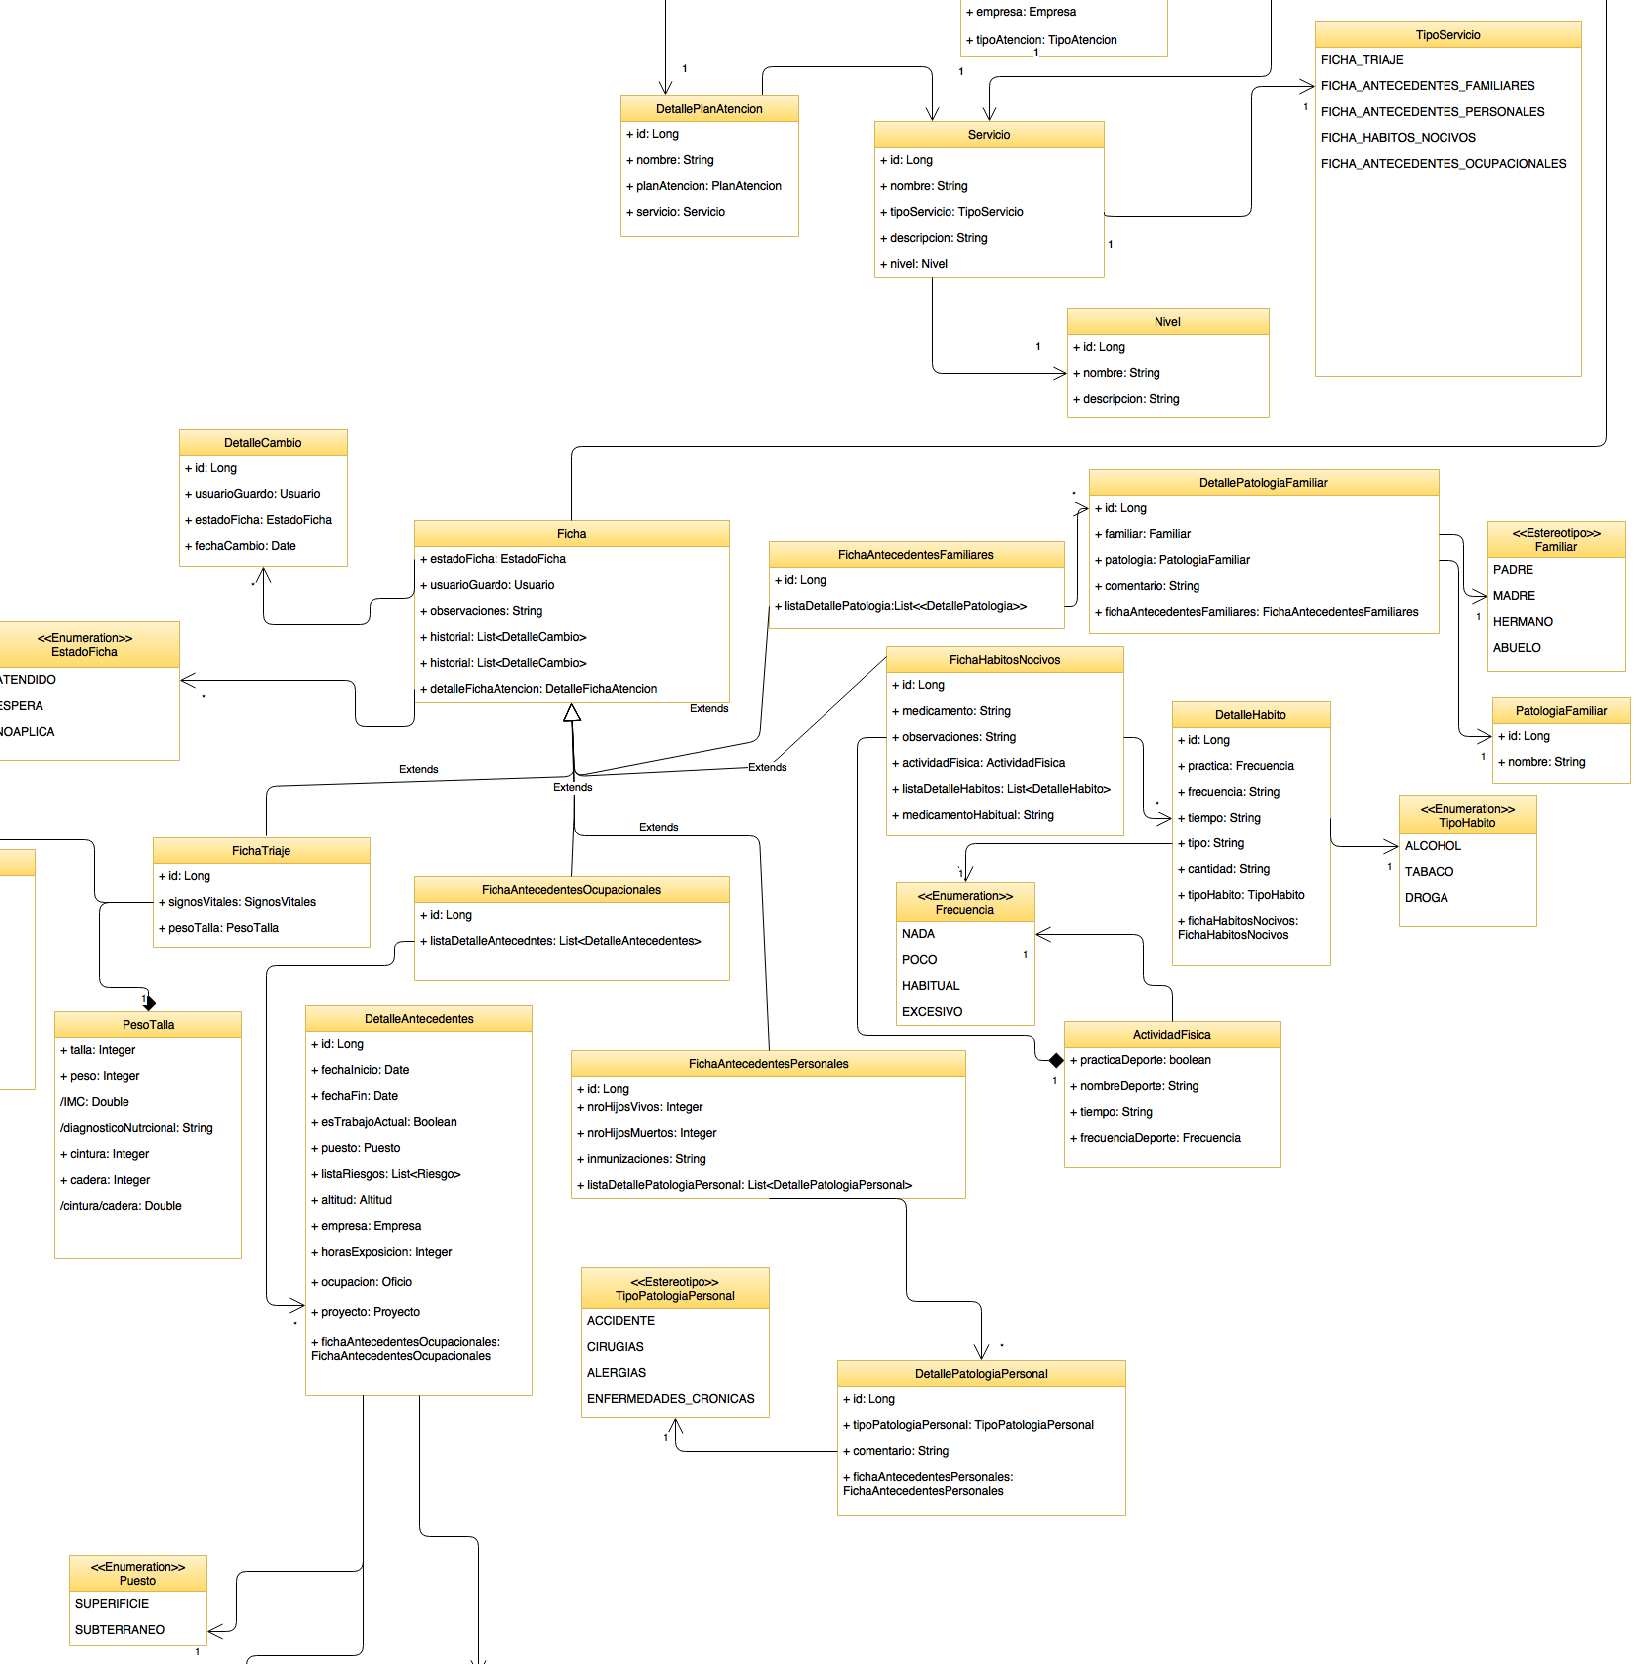
\includegraphics[width=17cm]{../imgs/disenio/DC2.png}
		\caption{DC-A Diagrama de clases}
	\end{figure}
	\begin{figure}[H]
	    \centering
		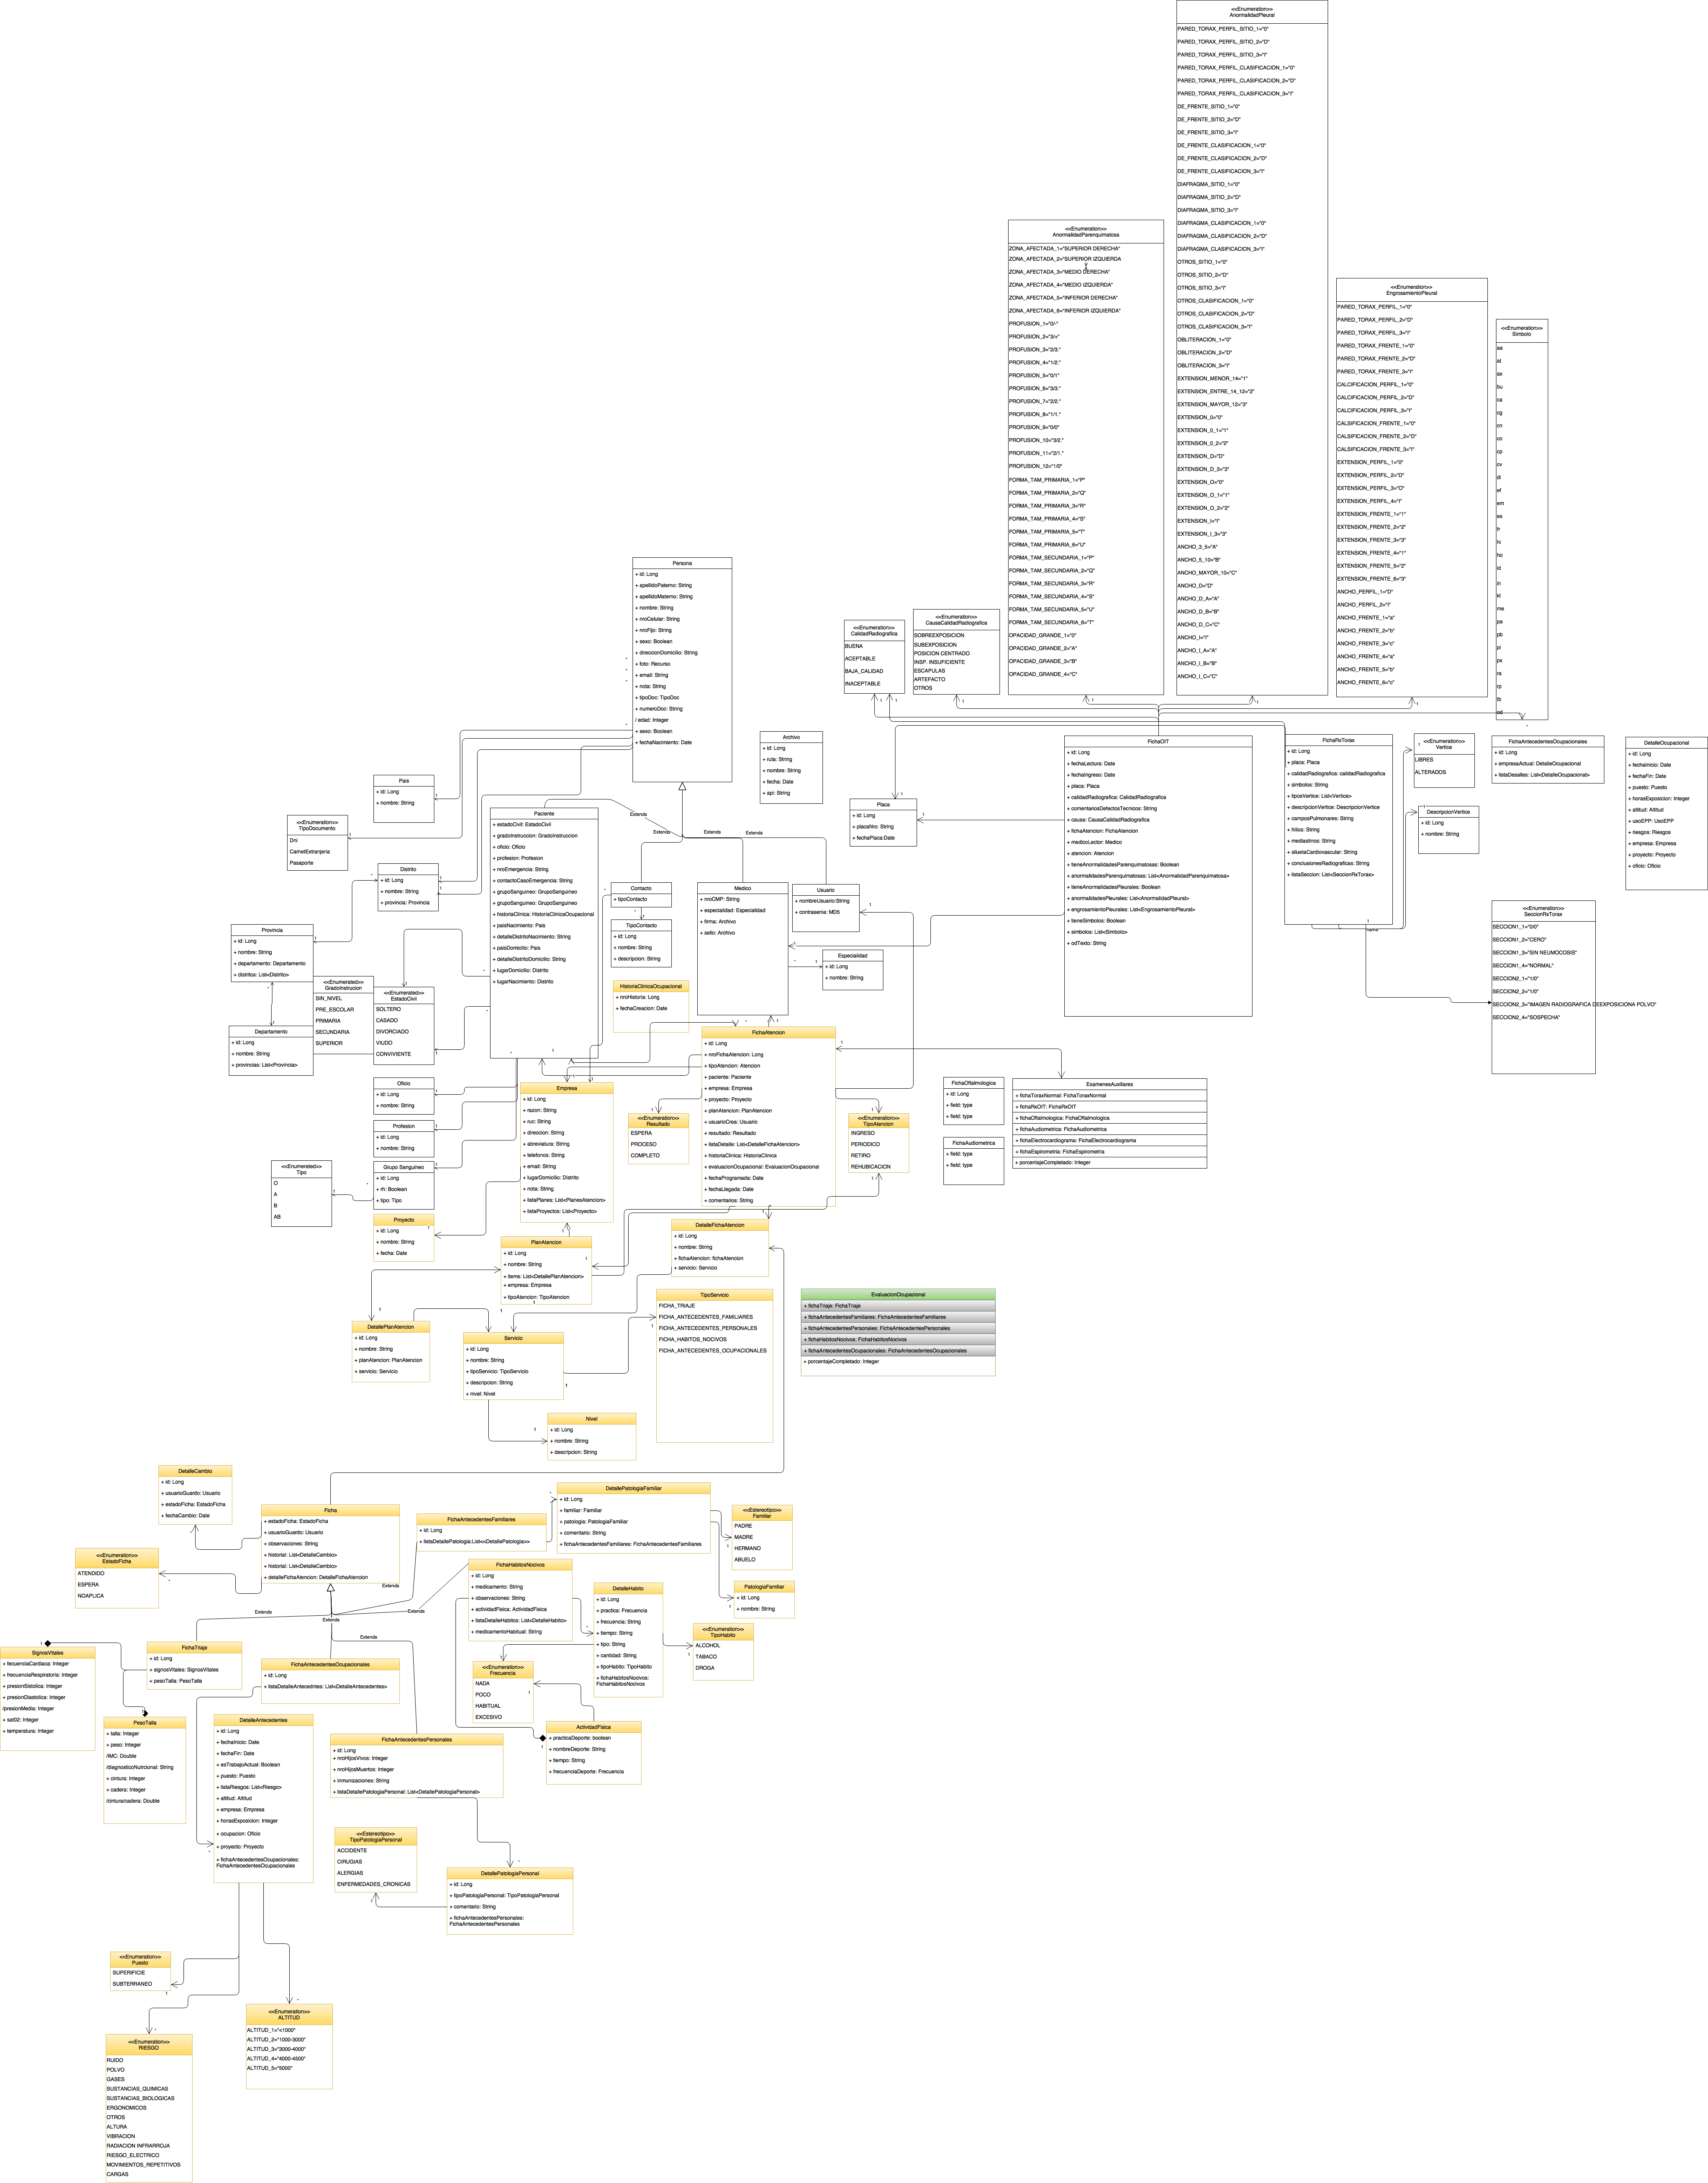
\includegraphics[width=18cm]{../imgs/disenio/DC.png}
		\caption{DC-B Diagrama de clases completo}
	\end{figure}
	\begin{figure}[H]
	    \centering
		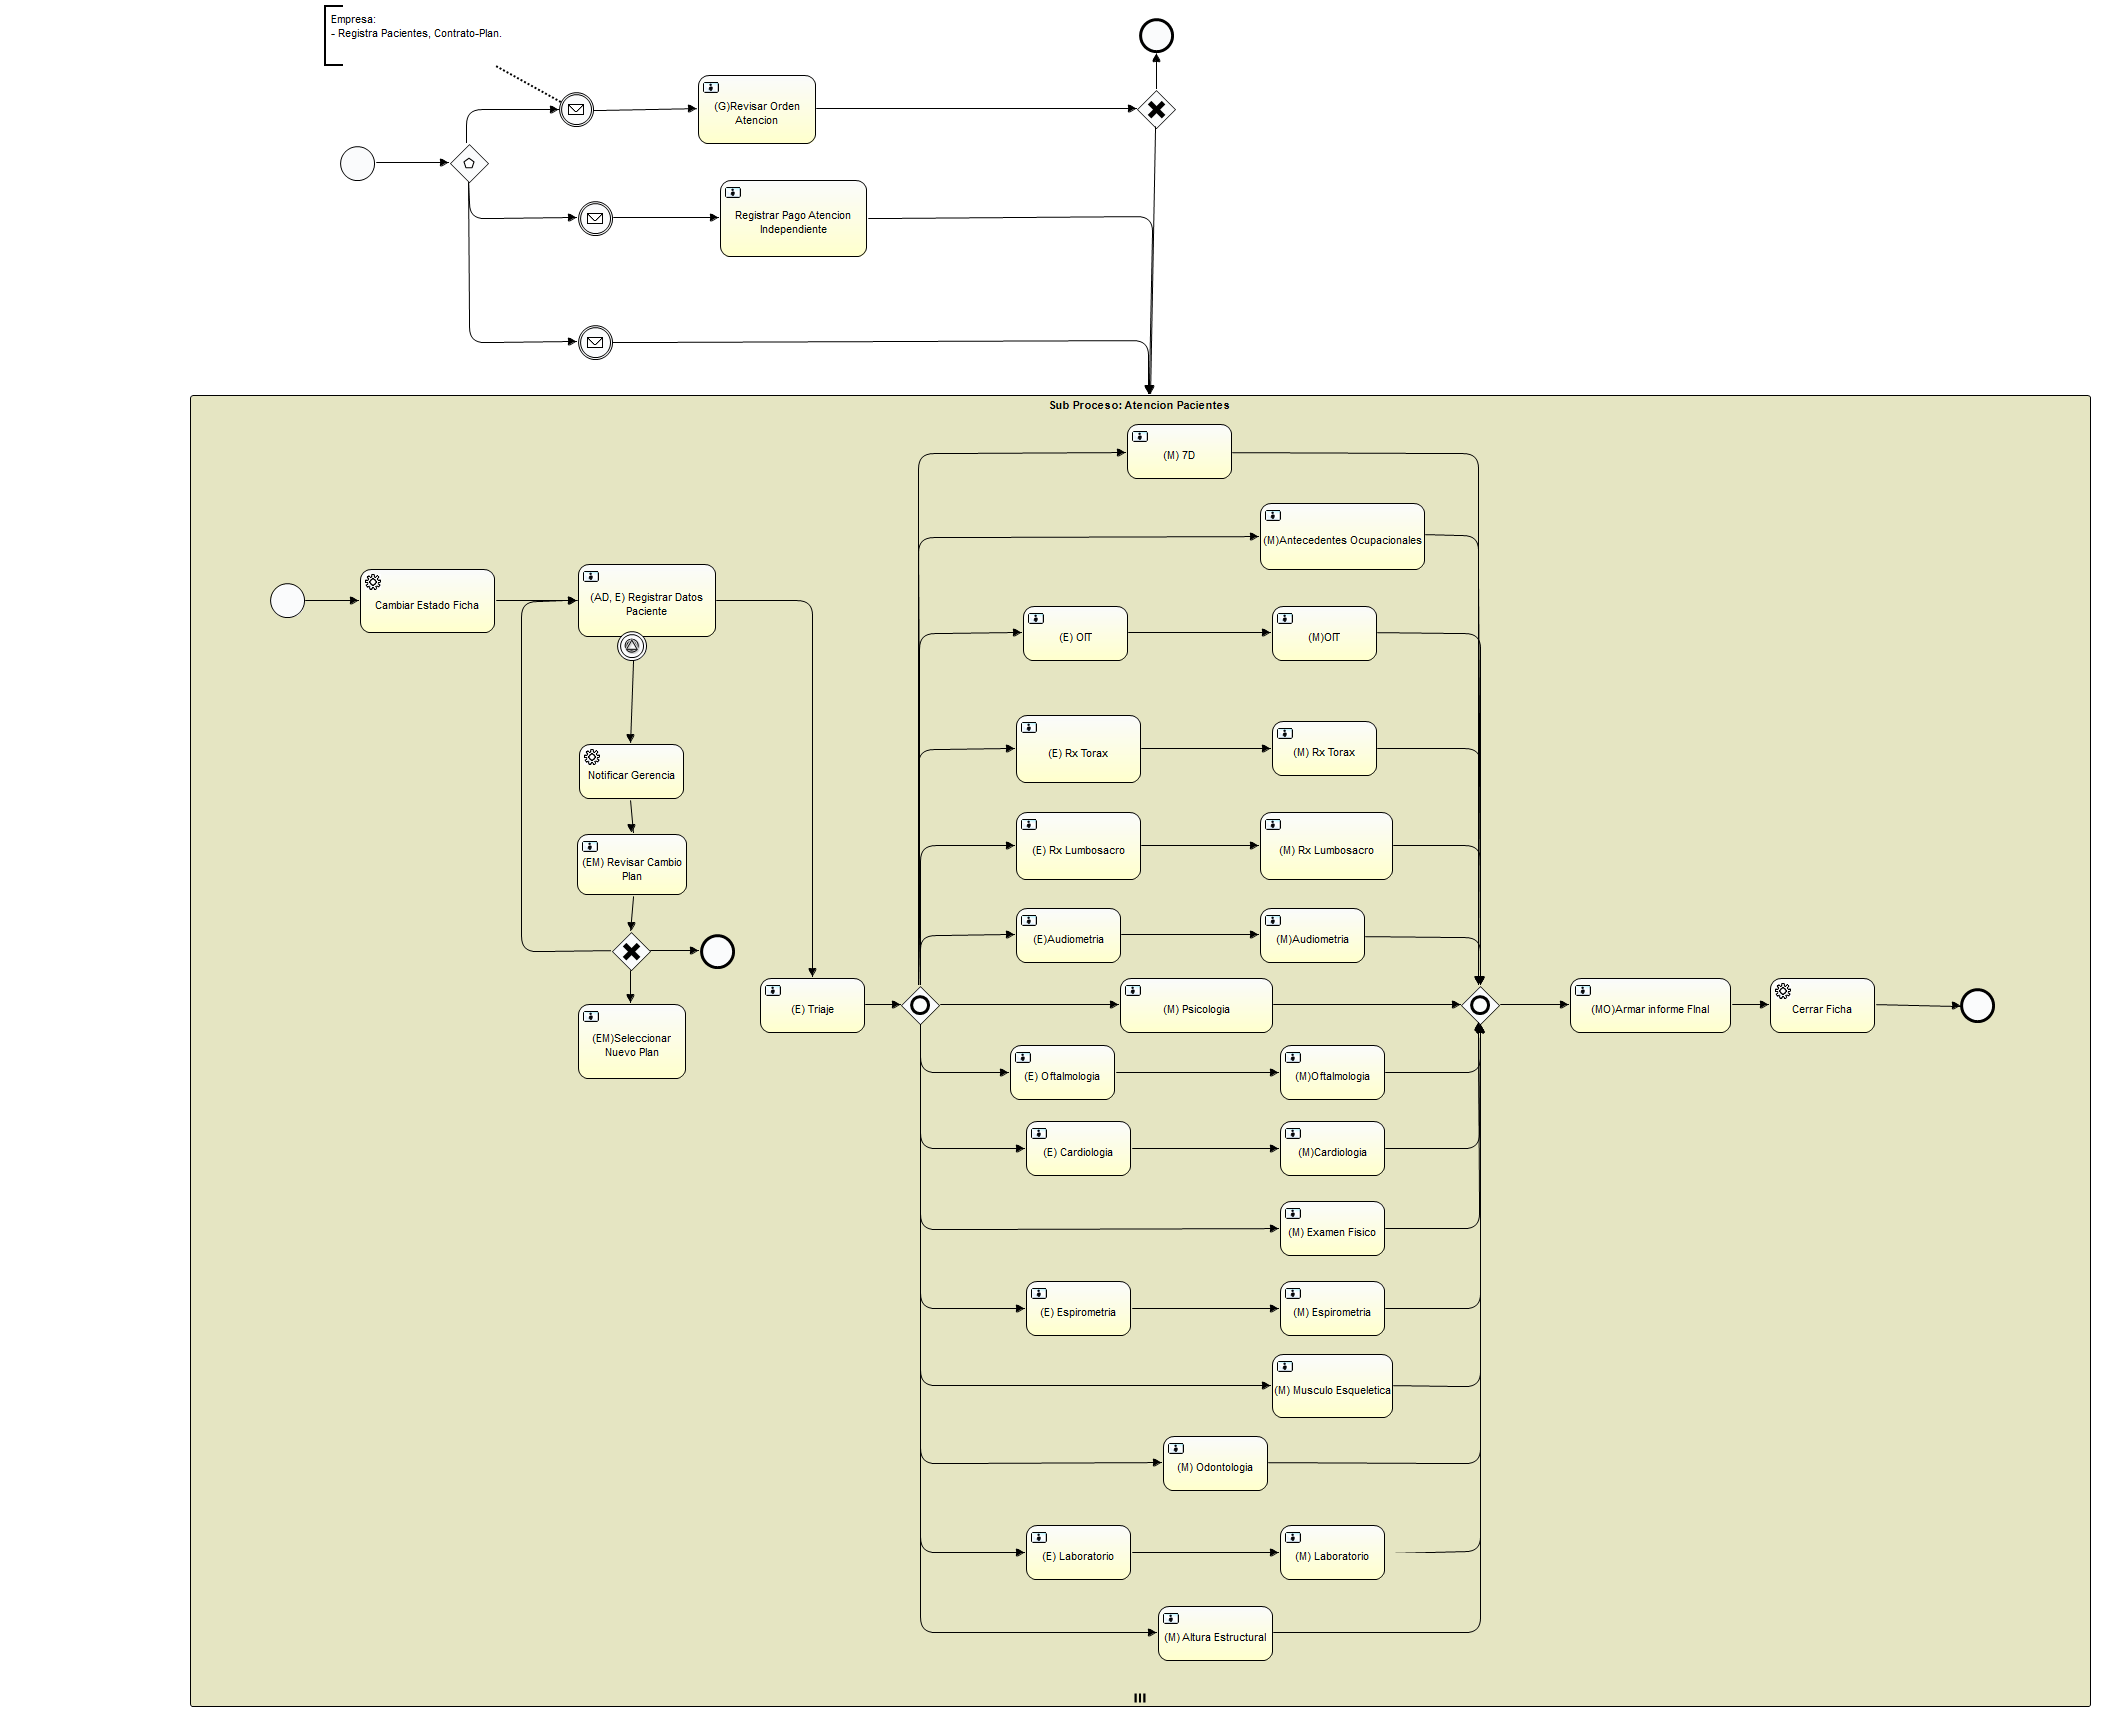
\includegraphics[width=18cm]{../imgs/disenio/ProcesoAtencion.png}
		\caption{DP-1 Diagrama BPM}
	\end{figure}
\newpage

\section{Arquitectura del Sistema}

	El Sistema sigue una arquitectura REST (Representational state trasfer) ó
	de servicios web RESTful cliente-servidor que, funciona bajo el protocolo
	HTTP, figura \ref{figure:arq1}. Básicamente el backend se encarga 
	de proporcionar recursos (previa autorización) al frontend.
	\\\
	
	\begin{figure}[ht!]
	    \centering
		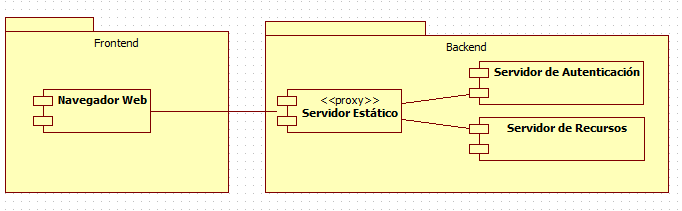
\includegraphics[width=18cm]{../imgs/disenio/arq1.png}
		\caption{DA-1 Arquitectura del Sistema}
		\label{figure:arq1}
	\end{figure}
	
	
	En la figura \ref{figure:arq2} se muestra detalladamente la interacción de los
	componentes (frontend y backend).
	\\\
	
	\begin{figure}[ht!]
	    \centering
		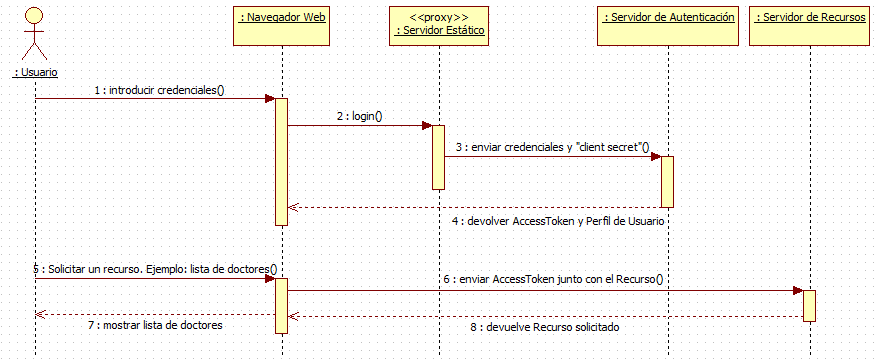
\includegraphics[width=18cm]{../imgs/disenio/arq2.png}
		\caption{DA-2 Arquitectura del Sistema (Diagrama de secuencia)}
		\label{figure:arq2}
	\end{figure}
		\section{Desarrollo del Sistema}
	
	Para el desarrollo del sistema se utilizó el siguiente stack de tecnologías
	(frontend y backend):
	
	\begin{itemize}
	  \item HTML y CSS (Bootstrap)
	  \item Javascript (AngularJS)
	  \item NodeJS (ExpressJS)
	  \item Java (Spring y Spring Boot)
	\end{itemize}
	
	\subsection{Arquitectura de Aplicaciones Web Modernas}
		A principios de la web, las ``aplicaciones web'' no existían. La web
  		consistía de contenido estático e imágenes.\\\
  
  		Ventajas:
  
  		\begin{itemize}
			\item Bajo consumo computacional en el servidor
			\item No se necesitan conocimientos avanzados en programación  
		\end{itemize}
		
		Desventajas:
		
		\begin{itemize}
			\item Actualización de contenido engorroso
			\item Personalización inexistente, todas las personas que visitan la web, ven
			el mismo contenido
			
			\item Interfaz de usuario muy básica, comparado con las aplicaciones actuales
		\end{itemize}
		
		Las aplicaciones web modernas estan compuestas de clientes frontend y una
		infraestructura backend distribuida (para servir contenido) a través del
		uso de APIs RESTful (figura \ref{figure:webapp-arq}).
		
		\begin{figure}[H]
		    \centering
			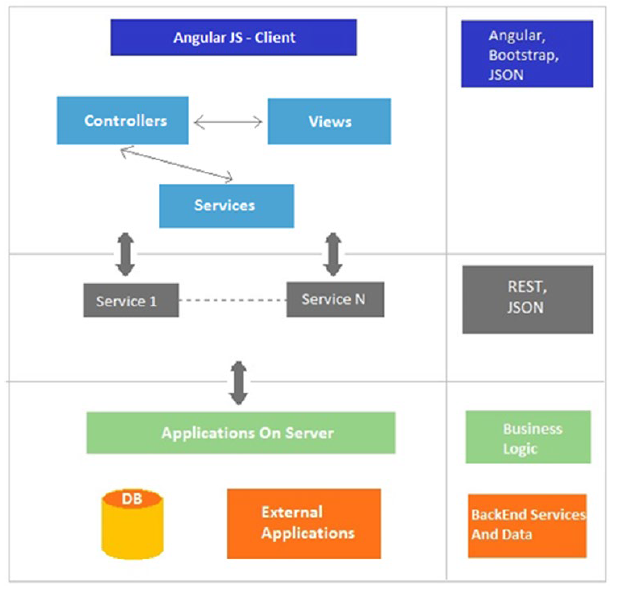
\includegraphics[width=16cm]{../imgs/ejemplos/webapp-arq.png}
			\caption{Arquitectura de aplicaciones web modernas}
			\label{figure:webapp-arq}
		\end{figure}
		
		 
	
	\subsection{Bootstrap}
		Bootstrap es un framework CSS que, facilita la creación se sitios web
		Responsive Web Design. Bootstrap viene con un conjunto de componentes de
		interfaz web listos para usar y una guía de estilos bastante completa,
		también provee grillas para el correcto maquetado de una web profesional.
		
		\begin{figure}[H]
		    \centering
			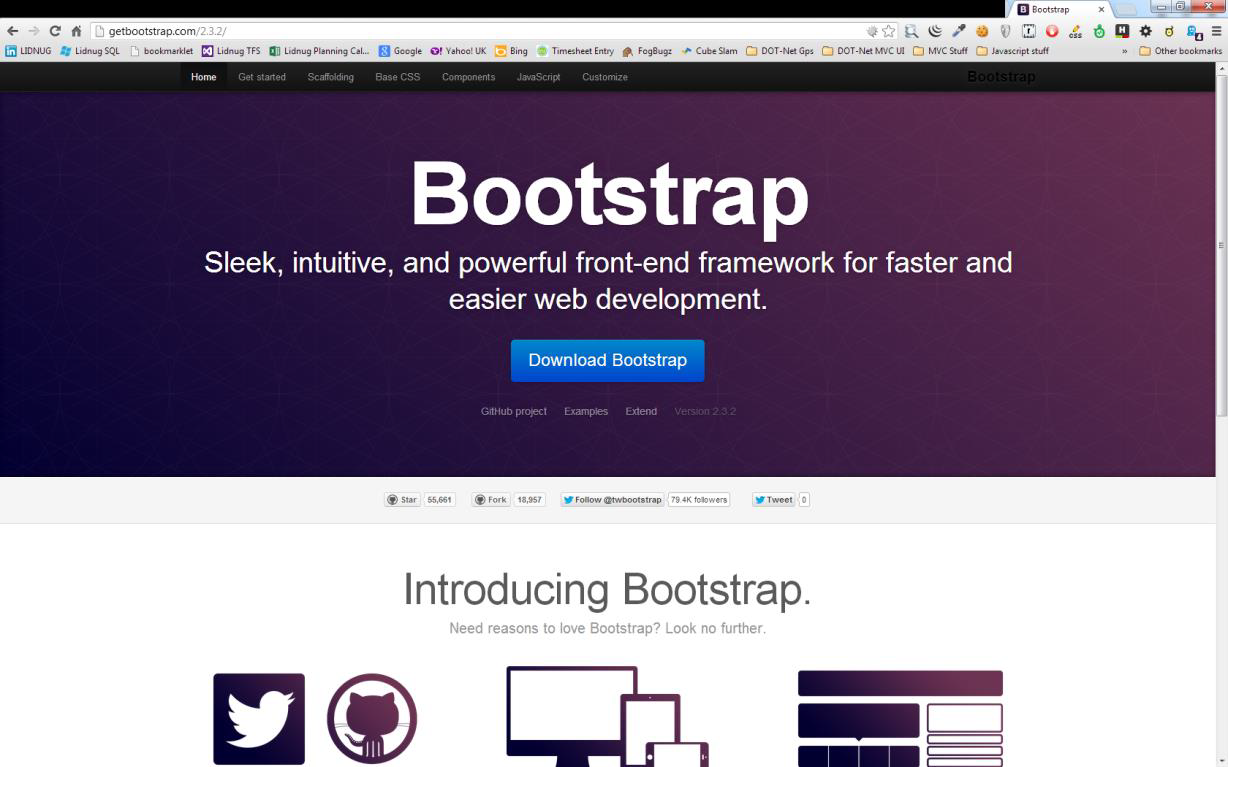
\includegraphics[width=17cm]{../imgs/ejemplos/bootstrap.png}
			\caption{Sitio Web de Bootstrap}
		\end{figure}
		
	
	\subsection{AngularJS}
		AngularJS es un framework de código abierto, soportado por Google. AngularJS
		permite a los desarrolladores crear aplicaciones web SPA (Single Page Applications), lo
		que facilita la experiencia de usuario, al no tener que cargar la
		aplicación web completa dos ó más veces.\\\
		
		A diferencia del las aplicaciones web SPA, en las aplicaciones
		web tradicionales (como se ilustra en la figura
		\ref{figure:carga-tradicional}), un cliente web hace una petición al servidor
		y éste responde con toda la página web completa; luego, el usuario hace click
		en un enlace interno, el servidor vuelve a cargar la página web completa
		y se produce un retraso en la carga de la página, lo que produce una mala
		experiencia de usuario.\footnote{Fuente de la imagen:
		\href{https://www.codeschool.com/course/shaping-up-with-angularjs}
		{https://www.codeschool.com/course/shaping-up-with-angularjs}} \\\
		
		\newpage
		
		\begin{figure}[H]
		    \centering
			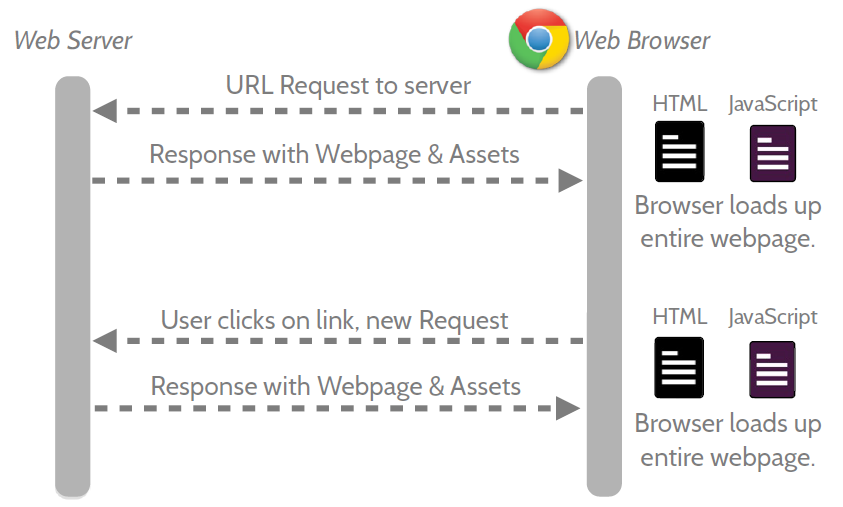
\includegraphics[width=18cm]{../imgs/ejemplos/1.png}
			\caption{Carga de página tradicional}
			\label{figure:carga-tradicional}
		\end{figure}
		
		
		En las aplicaciones SPA, el cliente solicita una web y el servidor
		inicialmente sirve la aplicación web completa (una sola vez); luego, el
		usuario hace click en un enlace interno, el servidor solo responde con el recurso
		solicitado, más no con la página web completa. En la figura
		\ref{figure:carga-spa} se muestra esta interacción.\footnote{Fuente de la imagen: 
		\href{https://www.codeschool.com/course/shaping-up-with-angularjs}
		{https://www.codeschool.com/course/shaping-up-with-angularjs}}
		
		\newpage
		\begin{figure}[H]
		    \centering
			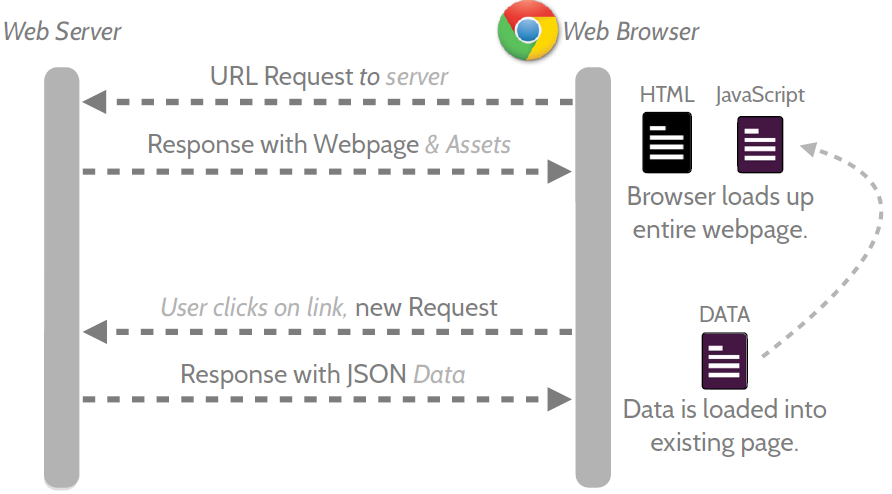
\includegraphics[width=18cm]{../imgs/ejemplos/2.png}
			\caption{Carga de página SPA}
			\label{figure:carga-spa}
		\end{figure}
		
		\newpage
		\subsubsection{Componentes}
			AngularJS ofrece una estructura modular y escalable para
			construir aplicaciones web, figura \ref{figure:angularjs-comp}.
			
			\begin{figure}[H]
			    \centering
				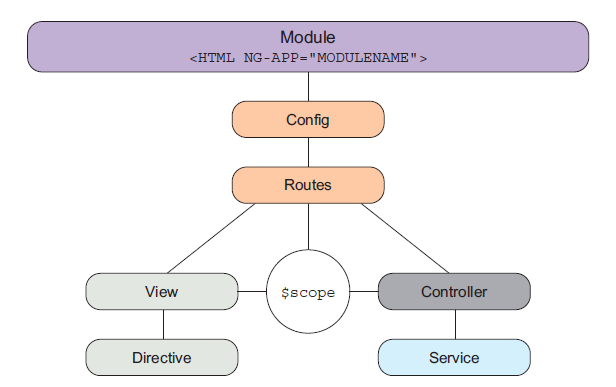
\includegraphics[width=18cm]{../imgs/ejemplos/angularjs-comp.png}
				\caption{Componentes de AngularJS}
				\label{figure:angularjs-comp}
			\end{figure}
			
			\begin{table}[H]
				\begin{tabular}{|p{2.75cm}|p{14cm}|} \hline
					 & \\
					\textit{\bfseries Componente} & \textit{\bfseries Propósito} \\
					 & \\ \hline
					 
					 & \\
					Module & Sirve como un contenedor que ayuda a organizar el
					código. Los Módulos pueden contener submódulos, haciendo fácil la
					composición de funcionalidades dentro de una aplicación web.\\
					 & \\
					 
					Config & El bloque de configuración permite ejecutar código javascript
					antes de que se ejecute la aplicación.\\
					 & \\
					
					Routes & Permite definir rutas para navegar a estados específicos de la
					aplicación.\\
					& \\
					
					View & La vista es la plantilla HTML que mostrará la aplicación.\\
					& \\
					
					\$scope & El \$scope es básicamente el pegamento entre la vista y el
					contralador\\
					& \\
					
					Controller & El controlador es responsable de la definición de métodos y
					propiedades. La vista es quien interactúa con el controlador.\\
					& \\
					
					Directive & Es una extensión de una vista, permite crear
					elementos HTML personalizados que encapsulan comportamientos.\\
					& \\
					Service & Proporcionan funcionalidades comunes a una aplicación.\\
					& \\ \hline
				\end{tabular}
				\caption{Resumen de componentes AngularJS}
			\end{table}
			
		\subsubsection{Arquitectura}
			AngularJS sigue una arquitectura MVC (Modelo-Vista-Controlador) para crear
			aplicaciones web. MVC es un patrón de
			arquitectura que separa los datos, lógica y
			presentación (figura \ref{figure:mvc}). Propuesto por
			\textit{Trygve Reenskaug} y después fue implementaado en el lenguaje de
			programación Smalltalk en los sententa \cite{scott1spa}.
			
			\begin{figure}[H]
			    \centering
				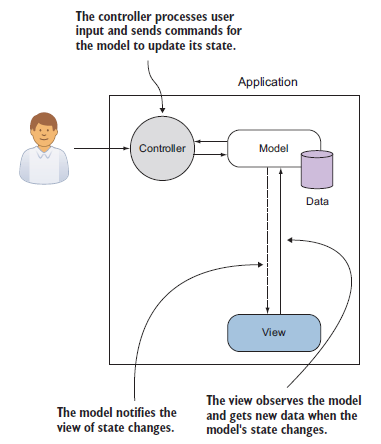
\includegraphics[width=16cm]{../imgs/ejemplos/mvc.png}
				\caption{Arquitectura Modelo-Vista-Controlador}
				\label{figure:mvc}
			\end{figure}
			
		
	\subsection{NodeJS y ExpressJS}
		NodeJS no es un lenguaje de programación, es una plataforma capaz de ejecutar
		aplicaciones complejas escritas en Javascript; se ejecuta en el lado del
		servidor como cualquier otro lenguaje (Java, Python, Ruby, etc).
		Para el sistema fue usado como un proxy, y a la vez como un servidor estático.\\\
		
		NodeJS está construido sobre el motor de javascript V8 creado por Google.
		NodeJS posee varias librerías escritas en C, junto con módulos para la
		manipulación de datos binarios. Puede acceder a funciones del sistema
		operativo, etc. Éstas librerías permiten a NodeJS acceder a archivos, ejecutar
		comandos del sistema, escuchar/responder a peticiones de red.\\\
		
		La figura \ref{figure:nodejs-comp} muestra los componentes principales de
		NodeJS:
		
		\begin{figure}[H]
		    \centering
			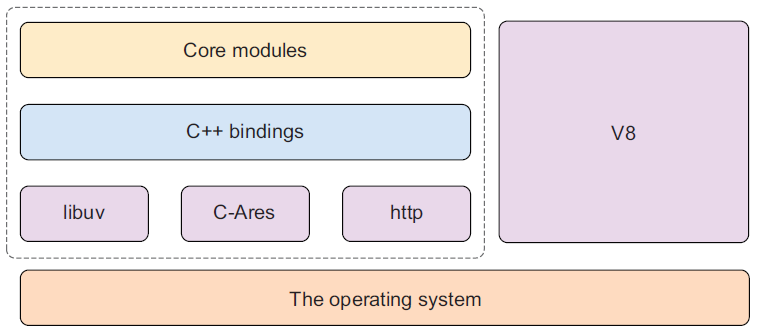
\includegraphics[width=16cm]{../imgs/ejemplos/nodejs-comp.png}
			\caption{Componentes de NodeJS}
			\label{figure:nodejs-comp}
		\end{figure}
		
		
		
		ExpressJS es un framework web para NodeJS. Proporciona una API sencilla de
		utilizar, y agiliza el desarrollo de proyectos backend.
	\newpage
	
	\subsection{Spring y Spring Boot}
		Spring es un framework java para el desarrollo de aplicaciones a nivel
		empresarial, inició como una alternativa liviana al estándar {\bf Java
		Enterprise Edition (JEE)}. Spring ofrece características como inyección de
		dependencias y un modelo de programación orientada a aspectos.\\\
		
		\subsubsection{Arquitectura}
			Como se muestra en la figura \ref{figure:spring-comp}, la arquitectura de
			Spring es modular, lo que permite elegir únicamente los módulos que
			necesitemos, sin necesidad de traer el framework completo.
		
			\begin{figure}[H]
			    \centering
				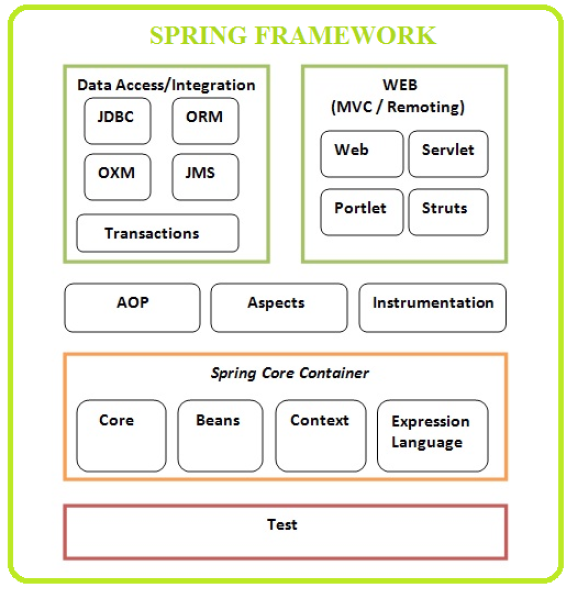
\includegraphics[width=14cm]{../imgs/ejemplos/spring-comp.png}
				\caption{Arquitectura de Spring Framework}
				\label{figure:spring-comp}
			\end{figure}
			
			
			
			\begin{table}[H]
				\begin{tabular}{|p{4.75cm}|p{12cm}|} \hline
					 & \\
					\textit{\bfseries Módulo} & \textit{\bfseries Propósito} \\
					 & \\ \hline
					 
					 & \\
					Core Container & Proporciona características de IoC (Inversión de Control)
					e Inyección de dependencias.\\
					 & \\
					 
					AOP \& Instrumentation & Proporciona un mecanimso para introducir nuevas
					funcionalidades a un código existente sin modificar su diseño.\\
					& \\
					
					Data Access/Integration & Se encarga de gestionar el acceso a bases de
					datos en una aplicación.\\
					& \\
					
					Web & Prorporciona un buen soporte para la creación de aplicaciones web
					robustas.\\
					& \\
					
					Test & Ayuda a realizar pruebas unitarias y de integración usando JUnit y
					TestNG.\\
					& \\
					
					& \\ \hline
				\end{tabular}
				\caption{Módulos de Spring}
			\end{table}
			
			
			
		
		Spring brinda muchas facilidades a la hora de programar, pero la
		configuración es un tanto compleja. Spring Boot simplifica todas las
		configuraciones iniciales para comenzar un proyecto web de manera rápida.
		Cabe mencionar que Spring Boot no es una herramienta ni una alternativa a Spring,
		es un proyecto que necesita de Spring para facilitarnos la vida.\\\
		
		Spring Boot trae algo de magia al desarrollo de aplicaciones con Spring.
		Existen cuatro características fundamentales:
		
		\begin{itemize}
		  \item {\bf Configuración Automática:} {Spring Boot
		  proporciona funcionalidades a nuestro proyecto de manera automática.}
		  
		  \item {\bf Dependencias Iniciales:} {De acuerdo al tipo de proyecto, Spring
		  Boot facilita las librerias necesarias para iniciar un proyecto.}
		  
		  \item {\bf Interfaz de Línea de Comandos:} {Esta característica opcional
		  permite escribir trozos de código directamente en la terminal e ir
		  probando funcionalidades.}
		  
		  \item {\bf Actuador (\textit{The Actuator}):} {Muestra características de
		  una aplicación en tiempo de ejecución.}
		\end{itemize}
		
		La página oficial (http://start.spring.io) del proyecto Spring Boot ofrece un
		asistente para la creación de proyectos utilizando maven o gradle:
		
		\begin{figure}[H]
		    \centering
			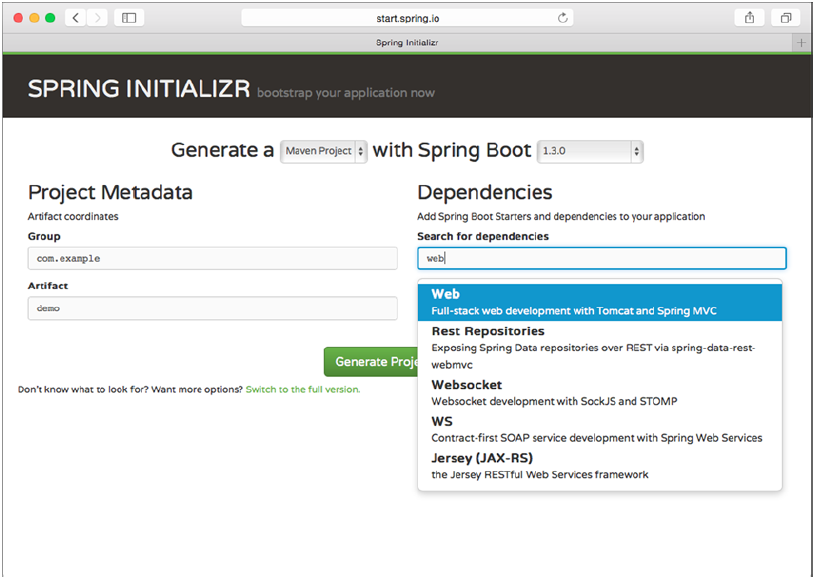
\includegraphics[width=14cm]{../imgs/ejemplos/spring-boot.png}
			\caption{Asistente de Spring Initializr}
			\label{figure:spring-boot}
		\end{figure}
		
		Después de generar el proyecto, obtenemos un archivo .zip el cual podemos
		importar a IDEs como Eclipse o NetBeans. La estructura de un proyecto Spring
		Boot es muy sencilla como se muestra en la figura
		\ref{figure:spring-boot-est}.

		\begin{figure}[H]
		    \centering
			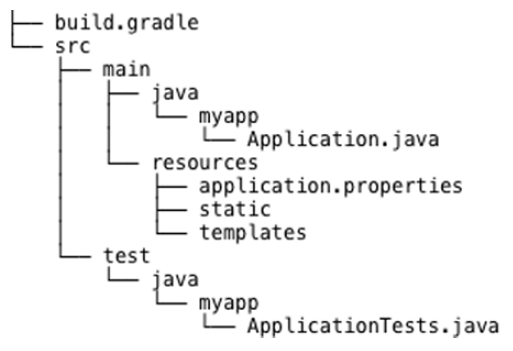
\includegraphics[width=10cm]{../imgs/ejemplos/spring-boot-est.png}
			\caption{Estructura de un proyecto Spring Boot}
			\label{figure:spring-boot-est}
		\end{figure}
		
		El ecosistema Spring cuenta con otros proyectos que vale la pena conocer, a
		continuación se listan algunos de ellos:
		
		\begin{table}[H]
			\begin{tabular}{|p{4.75cm}|p{12cm}|} \hline
				 & \\
				\textit{\bfseries Proyecto} & \textit{\bfseries Descripción} \\
				 & \\ \hline
				 
				 & \\
				Spring Cloud & Proporciona un conjunto de herramientas para sistemas
				distribuidos. Útil para la construcción y despliegue de microservicios.\\
				 & \\
				 
				Spring Data & Proporciona una aproximación consistente para el acceso a
				bases de datos: Relacionales, no-relacionales, map-reduce, etc.\\
				& \\
				
				Spring Batch & Simplifica y optimiza el procesamiento de altos volúmenes
				de operaciones en bloque.\\
				& \\
				
				Spring Security & Protege y asegura nuestras aplicaciones de una forma
				simple.
				Soporte para autenticación y autorización.\\
				& \\
				
				Spring Hateoas & Simplifica la creación de servicios RESTful y sigue el
				pricipio HATEOAS.\\
				& \\
				
				Spring Rest Docs & Documenta automáticamente nuestros servicios RESTful.\\
				& \\
				
				Spring Social & Conecta fácilmente nuestras aplicaciones con APIs de
				terceros: Facebook, Twitter, Linkedin y más.\\
				& \\
				
				& \\ \hline
			\end{tabular}
			\caption{Proyectos del ecosistema Spring}
		\end{table}
		
	
	\chapter{Conclusiones y Recomendaciones}
	
	\section{Conclusiones}
		\begin{itemize}
		  \item {Las prácticas realizadas en todo el proceso del desarrollo de software,
		obtención de requisitos, análisis de requisitos, diseño de sistemas,
		desarrollo e implementación; son actividades que el ingeniero de sistemas
		debe dominar, para realizar proyectos que ayuden a las personas y por ende a
		la sociedad.}

			\item {Uno de los obstáculos al que se enfrenta un prácticante es el de
			trabajar en equipo, transmitir ideas con claridad, pero que con la práctica
			se logra superar.}
			
			\item {La oportunidad que me dio la empresa {\bf WELL DONE SOLUTIONS SAC}, de
			hacerme partícipe en la construcción de un proyecto real desde un comienzo,
			fue un reto y que, además me fortaleció como ingeniero de sistemas. }
		\end{itemize}
		
	\section{Recomendaciones}
		\begin{itemize}
		  \item {Se recomienda a la empresa {\bf Well Done Solutions SAC} abra las
		  puertas a nuevos estudiantes quienes estén a punto de realizar sus
		  practicas pre profesionales, para que los futuros ingenieros de sistemas
		  estén muy bien capacitados.}
		  
		  \item {Se recomienda a la empresa {\bf Well Done Solutions SAC} brinde
		  talleres informativos a estudiantes de los distintos semestres de la
		  facultad de ingeniería de sistemas de esta casa de estudios.}
		  
		  \item {Se recomienda a la Carrera Académico Profesional de {\bf Ingeniería
		  de Sistemas} realizar convenios con empresas de  desarrollo de software, y así el estudiante
		  podrá enfrentarse a proyectos reales.}
		  
		  \item {Se recomienda a los estudiantes de la Carrera Académico Profesional de {\bf Ingeniería
		  de Sistemas} descargar este documento y su código fuente (hecho en {\LaTeX})
		  en el siguiente repositorio:
		  \href{https://www.github.com/w11ld33r}{https://www.github.com/w11ld33r}, para que puedan tener una noción de este informe y poder adecuarlo a sus necesidades.}
		  
		\end{itemize}
	\chapter{Anexos}	
		\section{Capturas de Pantalla de las contribuciones al código}
			A continuación se muestra las capturas de pantalla de algunas de las
			contribuciones al código fuente en el repositorio en la nube (Bitbucket):
			
			\begin{figure}[H]
			    \centering
				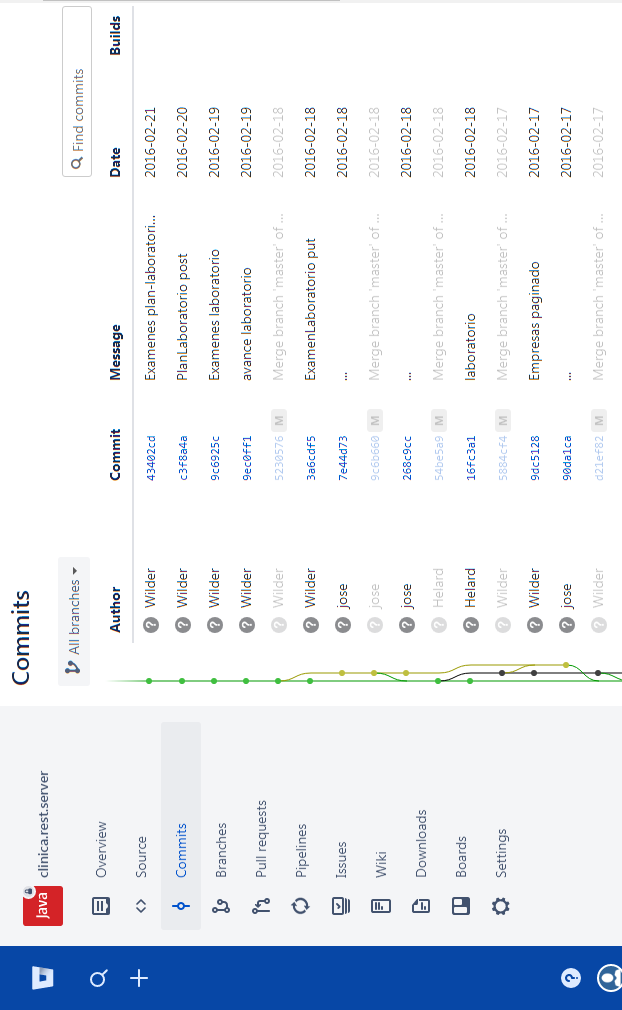
\includegraphics[width=13cm]{../imgs/ui/bitbucket-back.png}
				\caption{Pantalla contribución backend}
				\label{figure:bitbucket-back}
			\end{figure}
			
			\begin{figure}[H]
			    \centering
				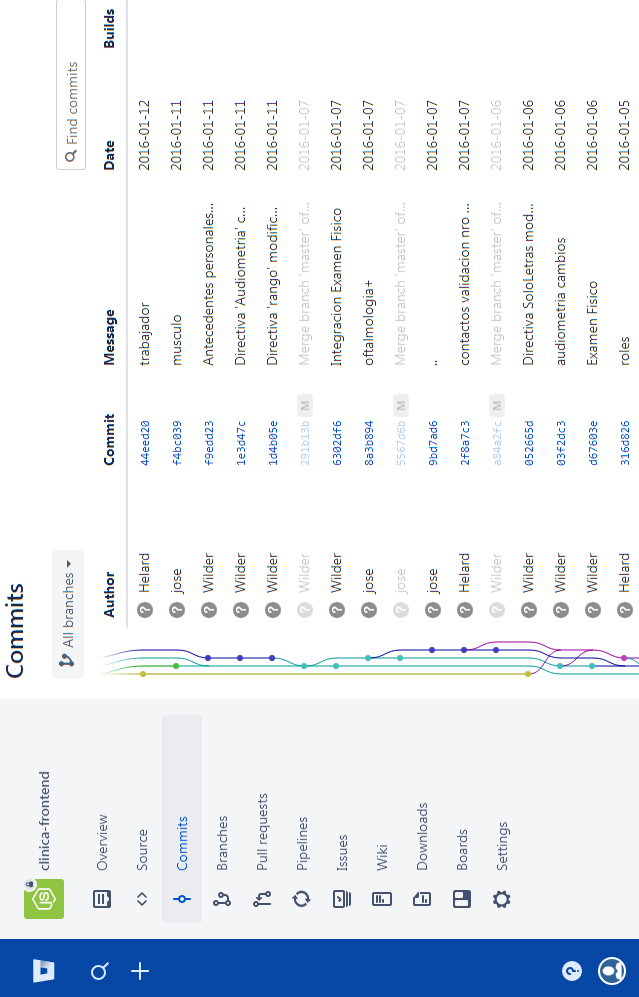
\includegraphics[width=13cm]{../imgs/ui/bitbucket-front.png}
				\caption{Pantalla contribución frontend}
				\label{figure:bitbucket-front}
			\end{figure}
		
		\section{Capturas de Pantalla del Sistema}
			A continuación se muestra algunas de las capturas de pantalla del sistema:
			
			\begin{figure}[H]
			    \centering
				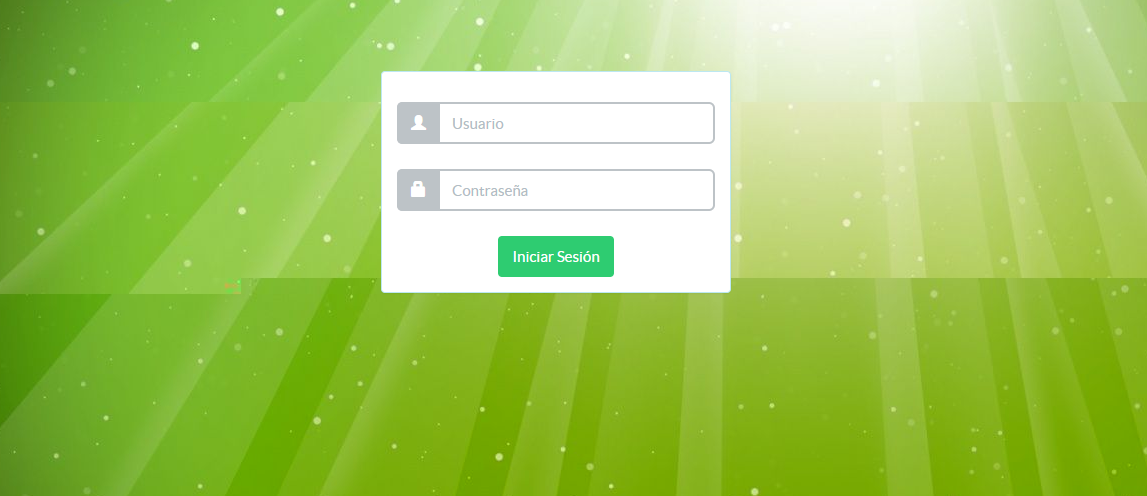
\includegraphics[width=18cm]{../imgs/ui/login.png}
				\caption{Pantalla login}
				\label{figure:login}
			\end{figure}
			
			\begin{figure}[H]
			    \centering
				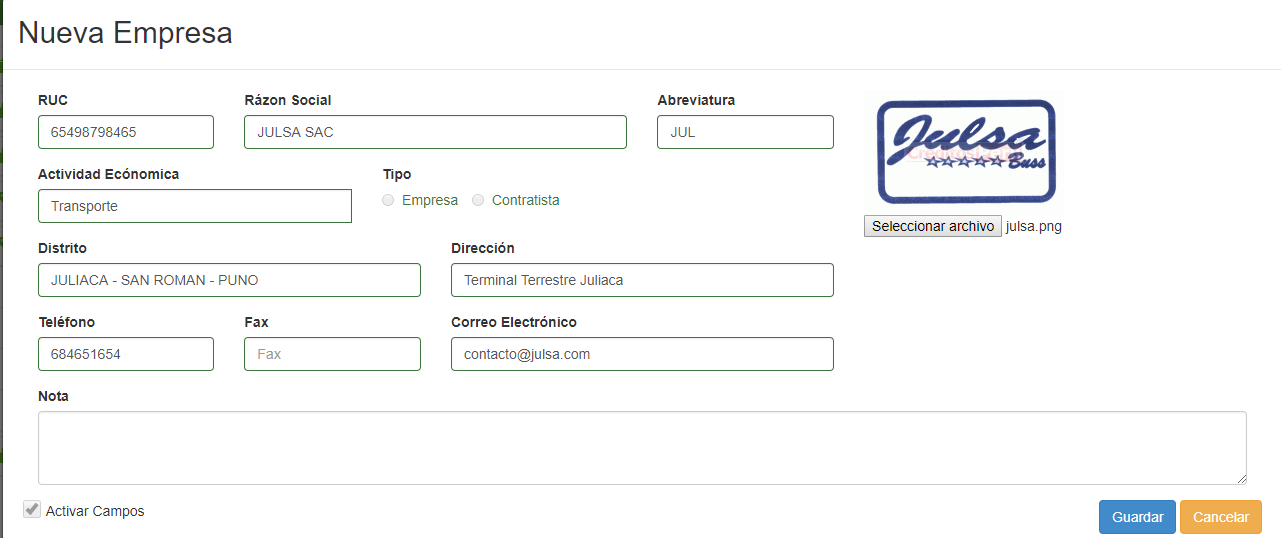
\includegraphics[width=18cm]{../imgs/ui/nueva-empresa.png}
				\caption{Pantalla nueva empresa}
				\label{figure:nueva-empresa}
			\end{figure}
			
			\begin{figure}[H]
			    \centering
				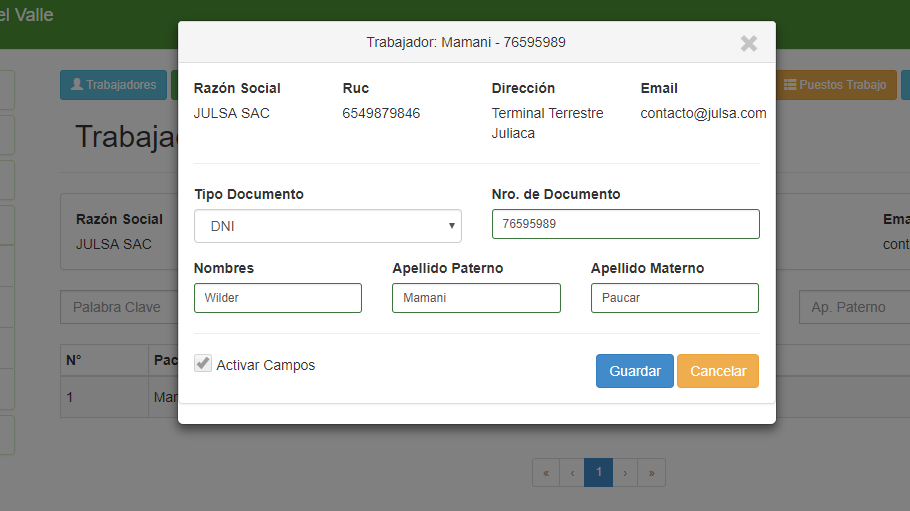
\includegraphics[width=18cm]{../imgs/ui/paciente.png}
				\caption{Pantalla nuevo paciente}
				\label{figure:paciente}
			\end{figure}
			
			\begin{figure}[H]
			    \centering
				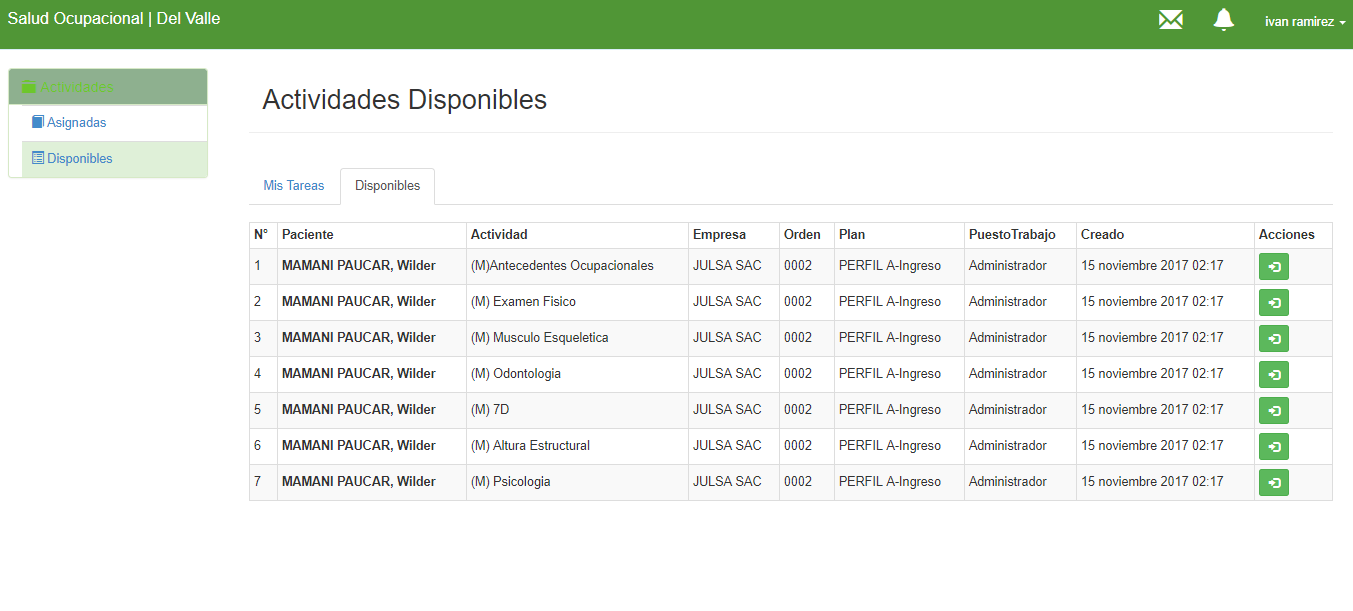
\includegraphics[width=18cm]{../imgs/ui/disponibles.png}
				\caption{Pantalla exámenes a realizar}
				\label{figure:disponibles}
			\end{figure}
			
			\begin{figure}[H]
			    \centering
				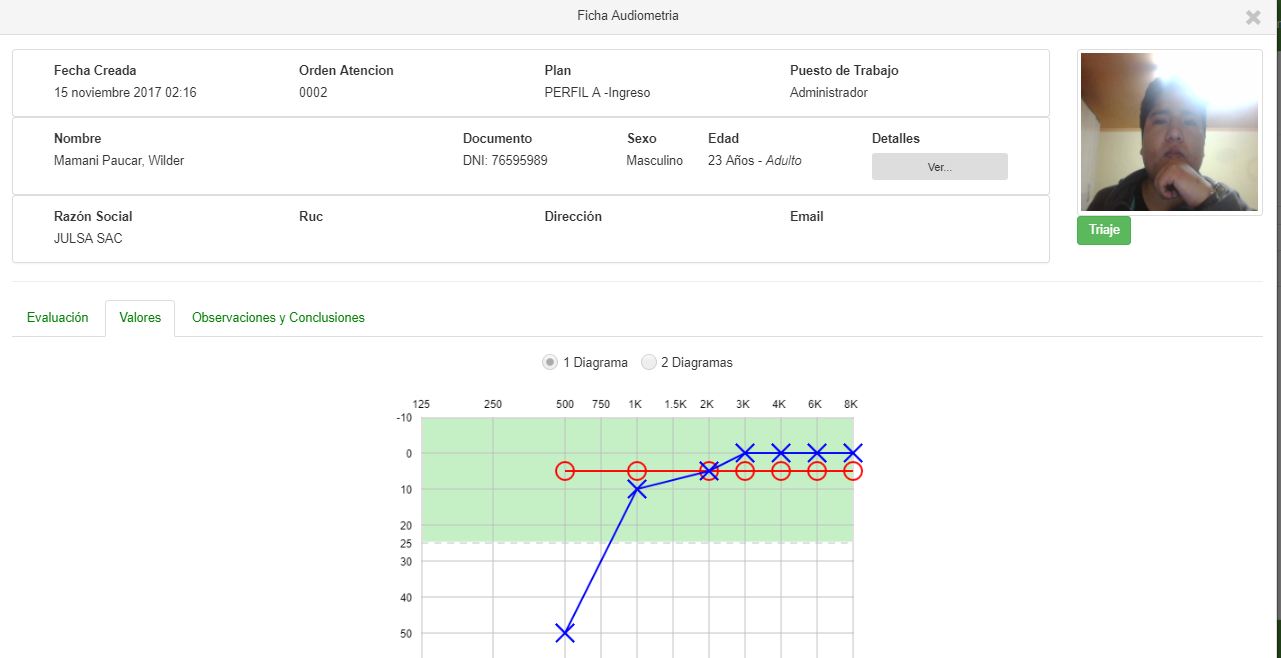
\includegraphics[width=18cm]{../imgs/ui/audiometria.png}
				\caption{Pantalla examen audiometría}
				\label{figure:audiometria}
			\end{figure}
			
			\begin{figure}[H]
			    \centering
				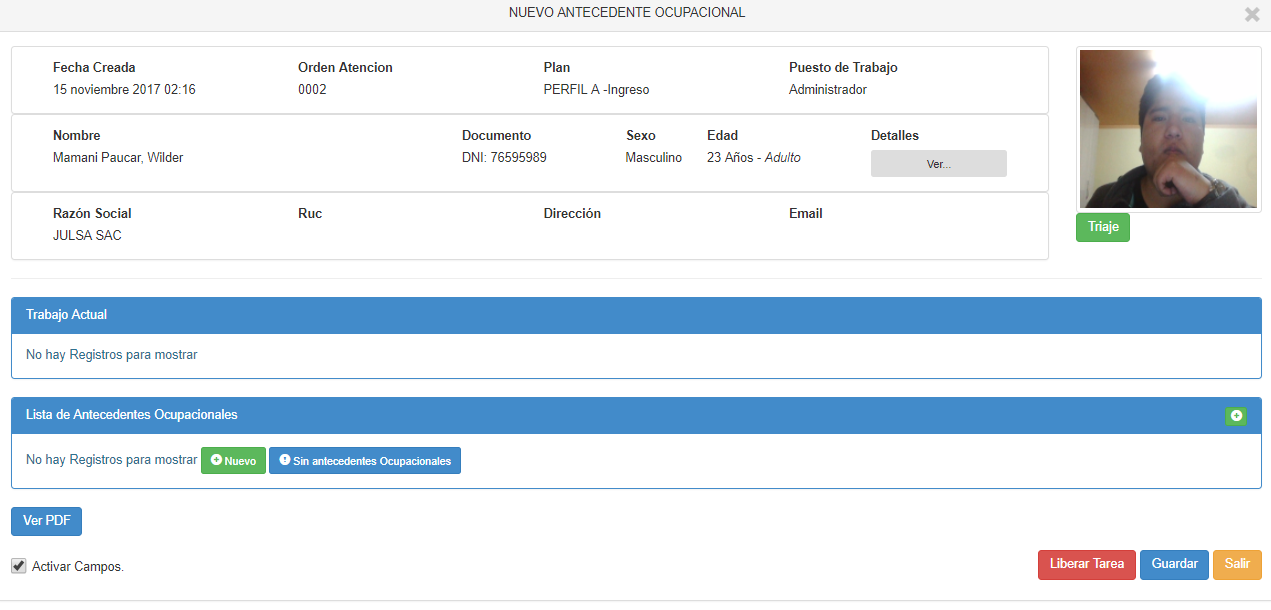
\includegraphics[width=18cm]{../imgs/ui/ocupacional.png}
				\caption{Pantalla antecedentes ocupacionales}
				\label{figure:ocupacional}
			\end{figure}
			
			
			
		\section{Capturas de Pantalla del Código}
			A continuación se muestra algunas de las capturas de pantalla del código
			fuente (frontend y backend:
			
			\begin{figure}[H]
			    \centering
				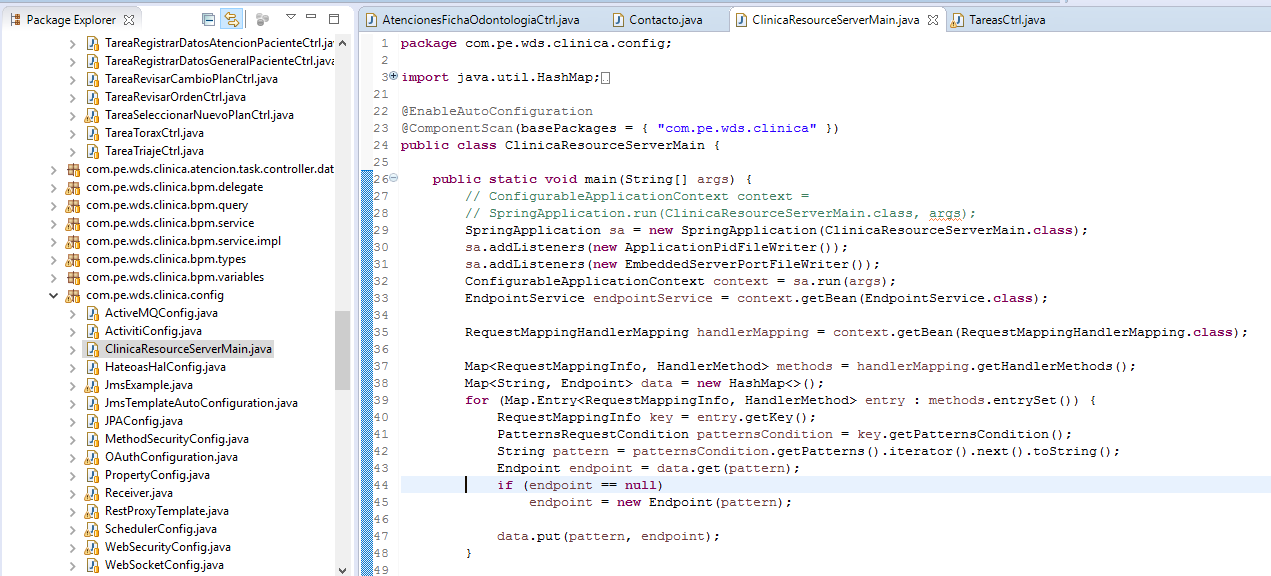
\includegraphics[width=18cm]{../imgs/codigo/back-main.png}
				\caption{Pantalla backend código principal}
				\label{figure:back-main}
			\end{figure}
			
			\begin{figure}[H]
			    \centering
				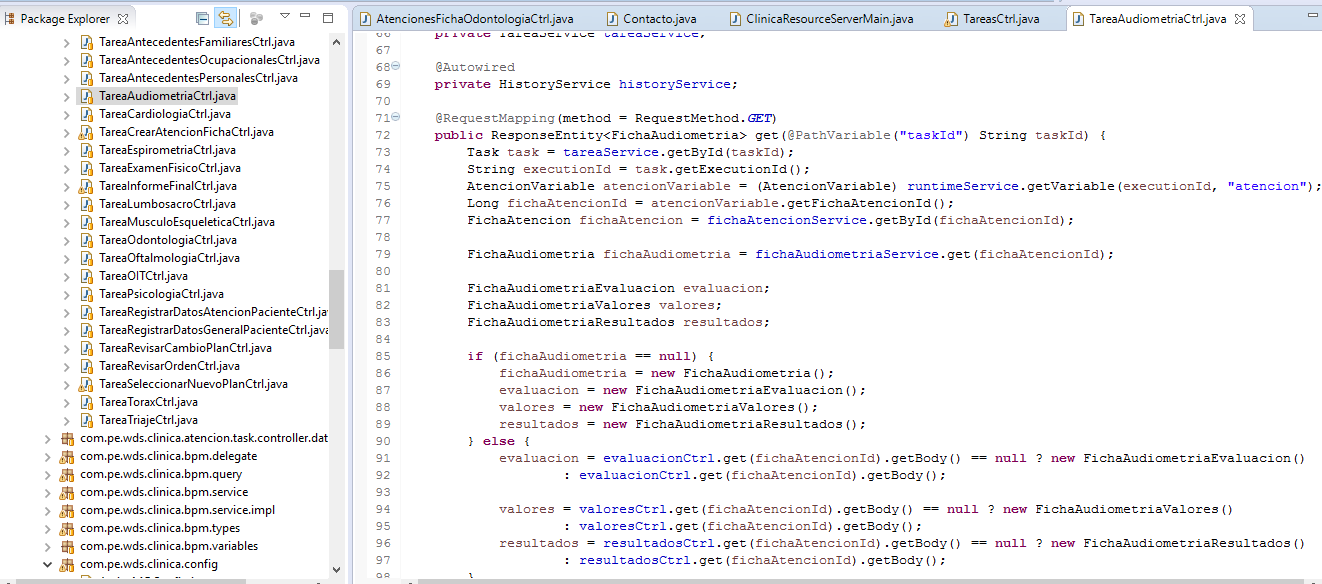
\includegraphics[width=18cm]{../imgs/codigo/back-ctrl.png}
				\caption{Pantalla backend código controlador audiometría}
				\label{figure:back-ctrl}
			\end{figure}
			
			
			\begin{figure}[H]
			    \centering
				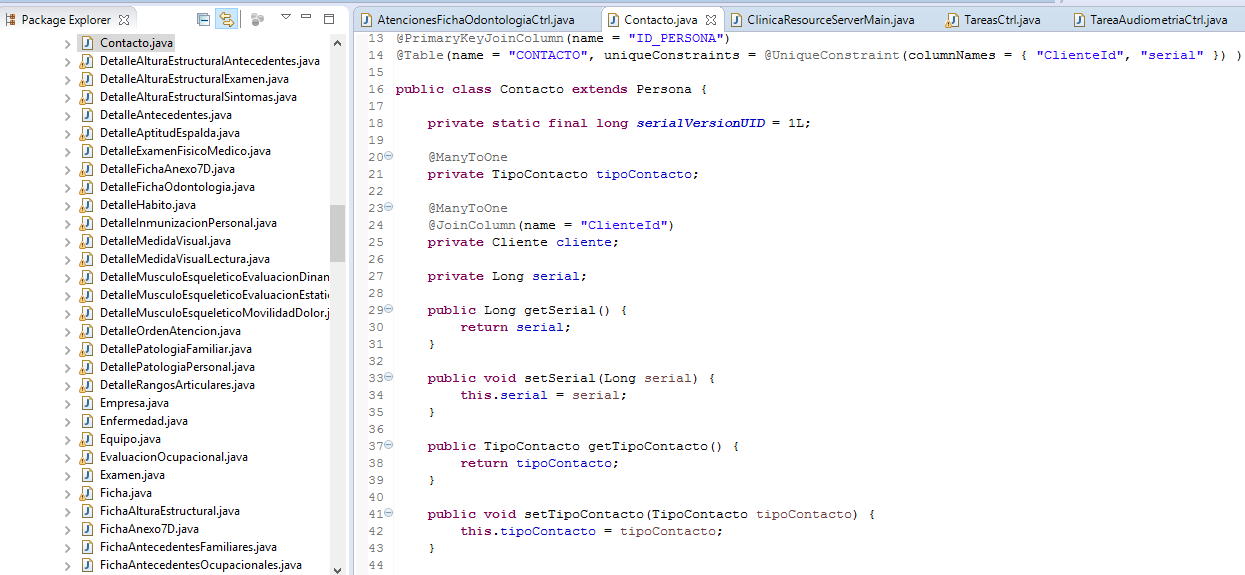
\includegraphics[width=18cm]{../imgs/codigo/back-entity.png}
				\caption{Pantalla backend código entidad contacto}
				\label{figure:back-entity}
			\end{figure}
			
			\begin{figure}[H]
			    \centering
				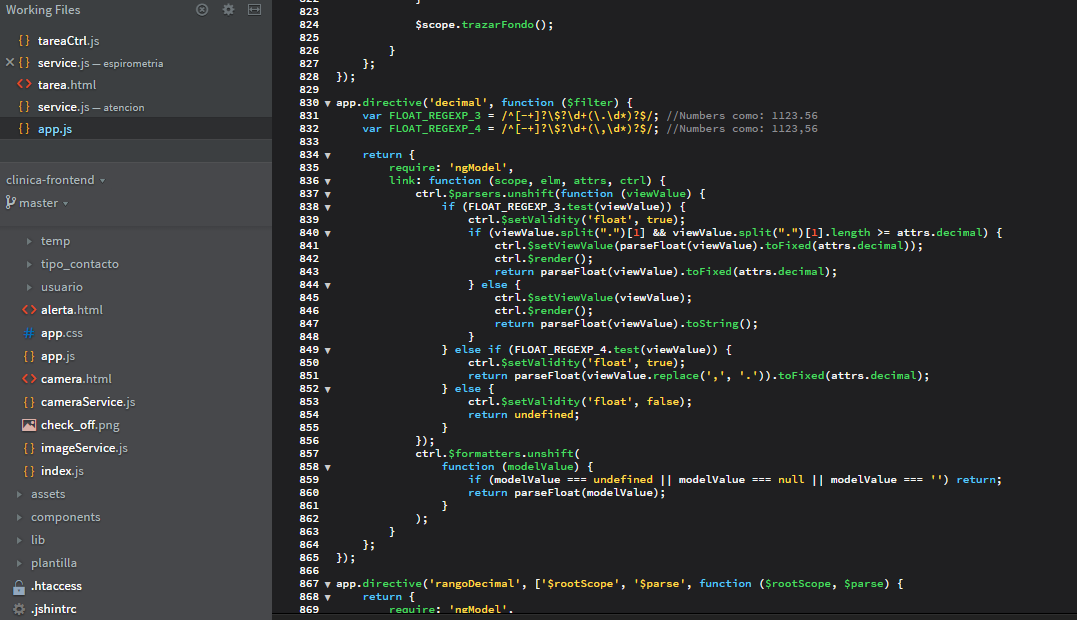
\includegraphics[width=18cm]{../imgs/codigo/front-main.png}
				\caption{Pantalla frontend código principal}
				\label{figure:front-main}
			\end{figure}
			
			\begin{figure}[H]
			    \centering
				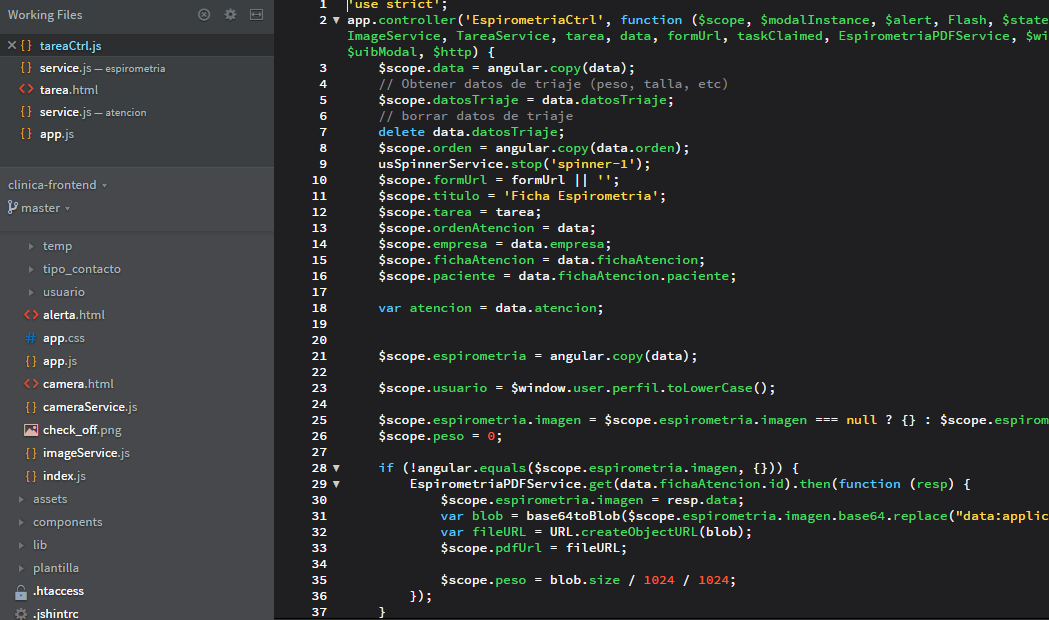
\includegraphics[width=16cm]{../imgs/codigo/front-ctrl.png}
				\caption{Pantalla frontend código controlador espirometría}
				\label{figure:front-ctrl}
			\end{figure}
			
			\begin{figure}[H]
			    \centering
				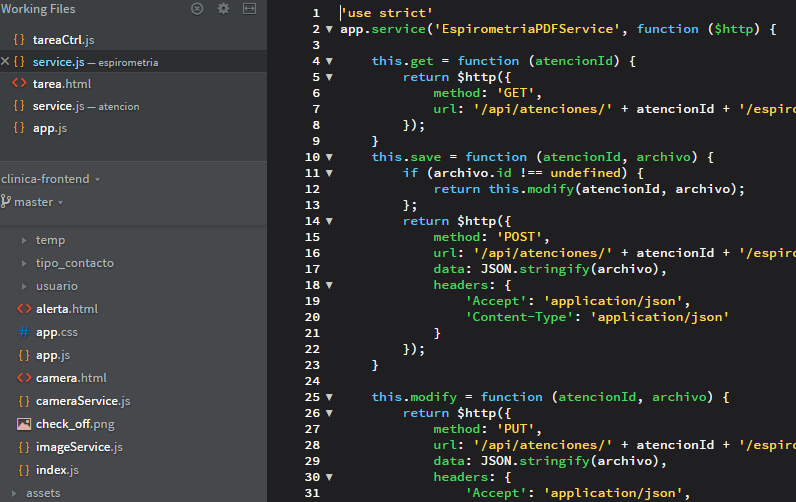
\includegraphics[width=15cm]{../imgs/codigo/front-service.png}
				\caption{Pantalla frontend código comunicación con el backend}
				\label{figure:front-service}
			\end{figure}
	
	\bibliographystyle{apalike}
	\bibliography{bib}
	\nocite{*}

\end{document}

